%%%%%%%%%%%%%%%%%%don't forget if needed %%%%%%%%%%%%%%%%%%%%%
%\section[toc version]{title version%
%              \sectionmark{head version}}
%\sectionmark{head version}
%%%%%%%%%%%%%%%%%%%%%%%%%%%%%%%%%%%%%%%%%%%%%%%%%%%%%%%%%%%%%%
\def\titcourt{Numerical comparison of basal and lateral melting of phase change materials}
\def\titlong{Numerical comparison of basal and lateral melting of phase change materials}
%%%%%%%%%%%%%%%%%%%%%%%%%%%%%%%%%%%%%%%%%%%%%%%%%%%%%%%%%%%%%%%%
\chapter[\titlong]{\titlong%
              \chaptermark{\titcourt}}
\chaptermark{\titcourt}
\label{chap-MELTING-CAVITY}
%%%%%%%%%%%%%%%%%%%%%%%%%%%%%%%%%%%%%%%%%%%%%%%%%%%%%%%%%%%%%%%%
%%%%%%%%%%%%%%%%%%%%%%%%%%%%%%%%%%%%%%%%%%%%%%%%%%%%%%%%%%%%%%%%
\begin{figure}
	\begin{center}
		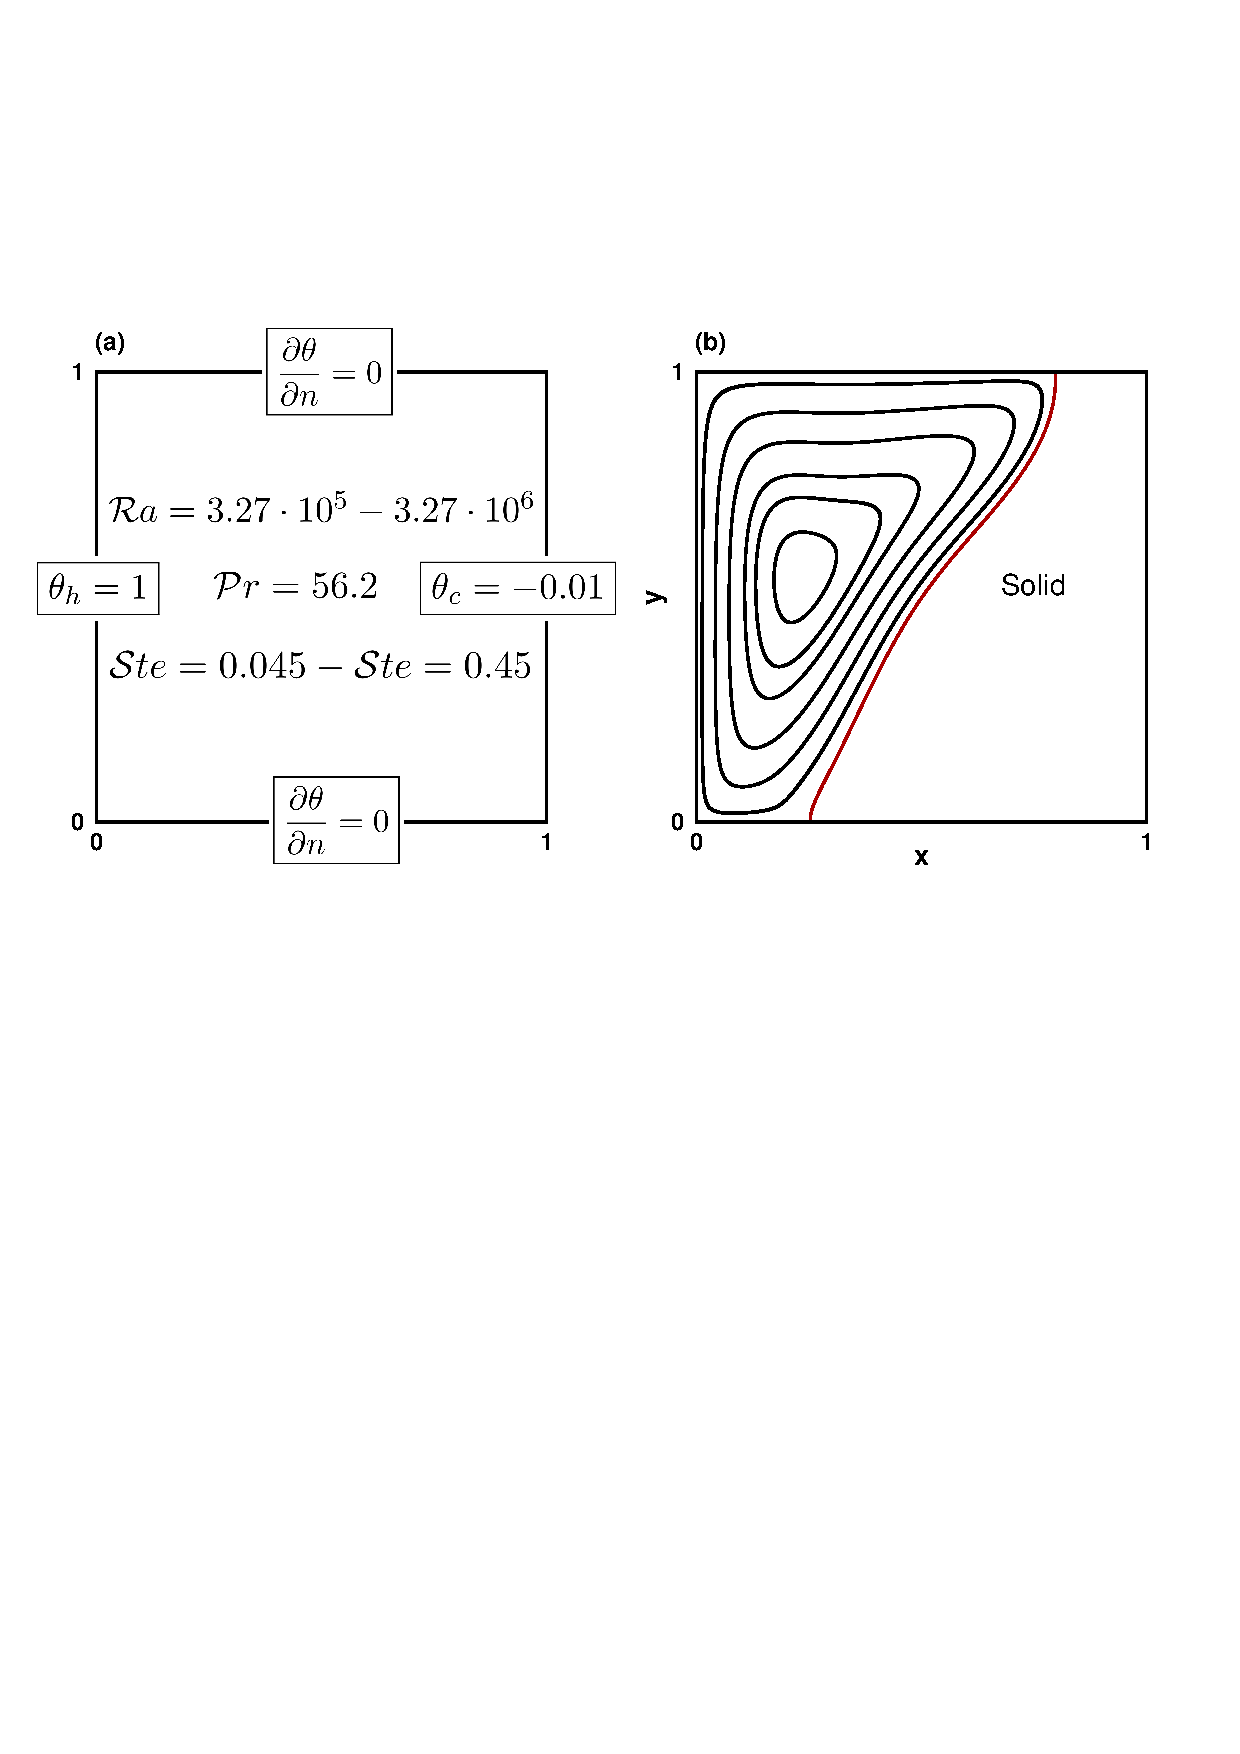
\includegraphics[width=\textwidth]{\figpath/Fig_cap_melting_basal/Scheme-melt-lat} \\
		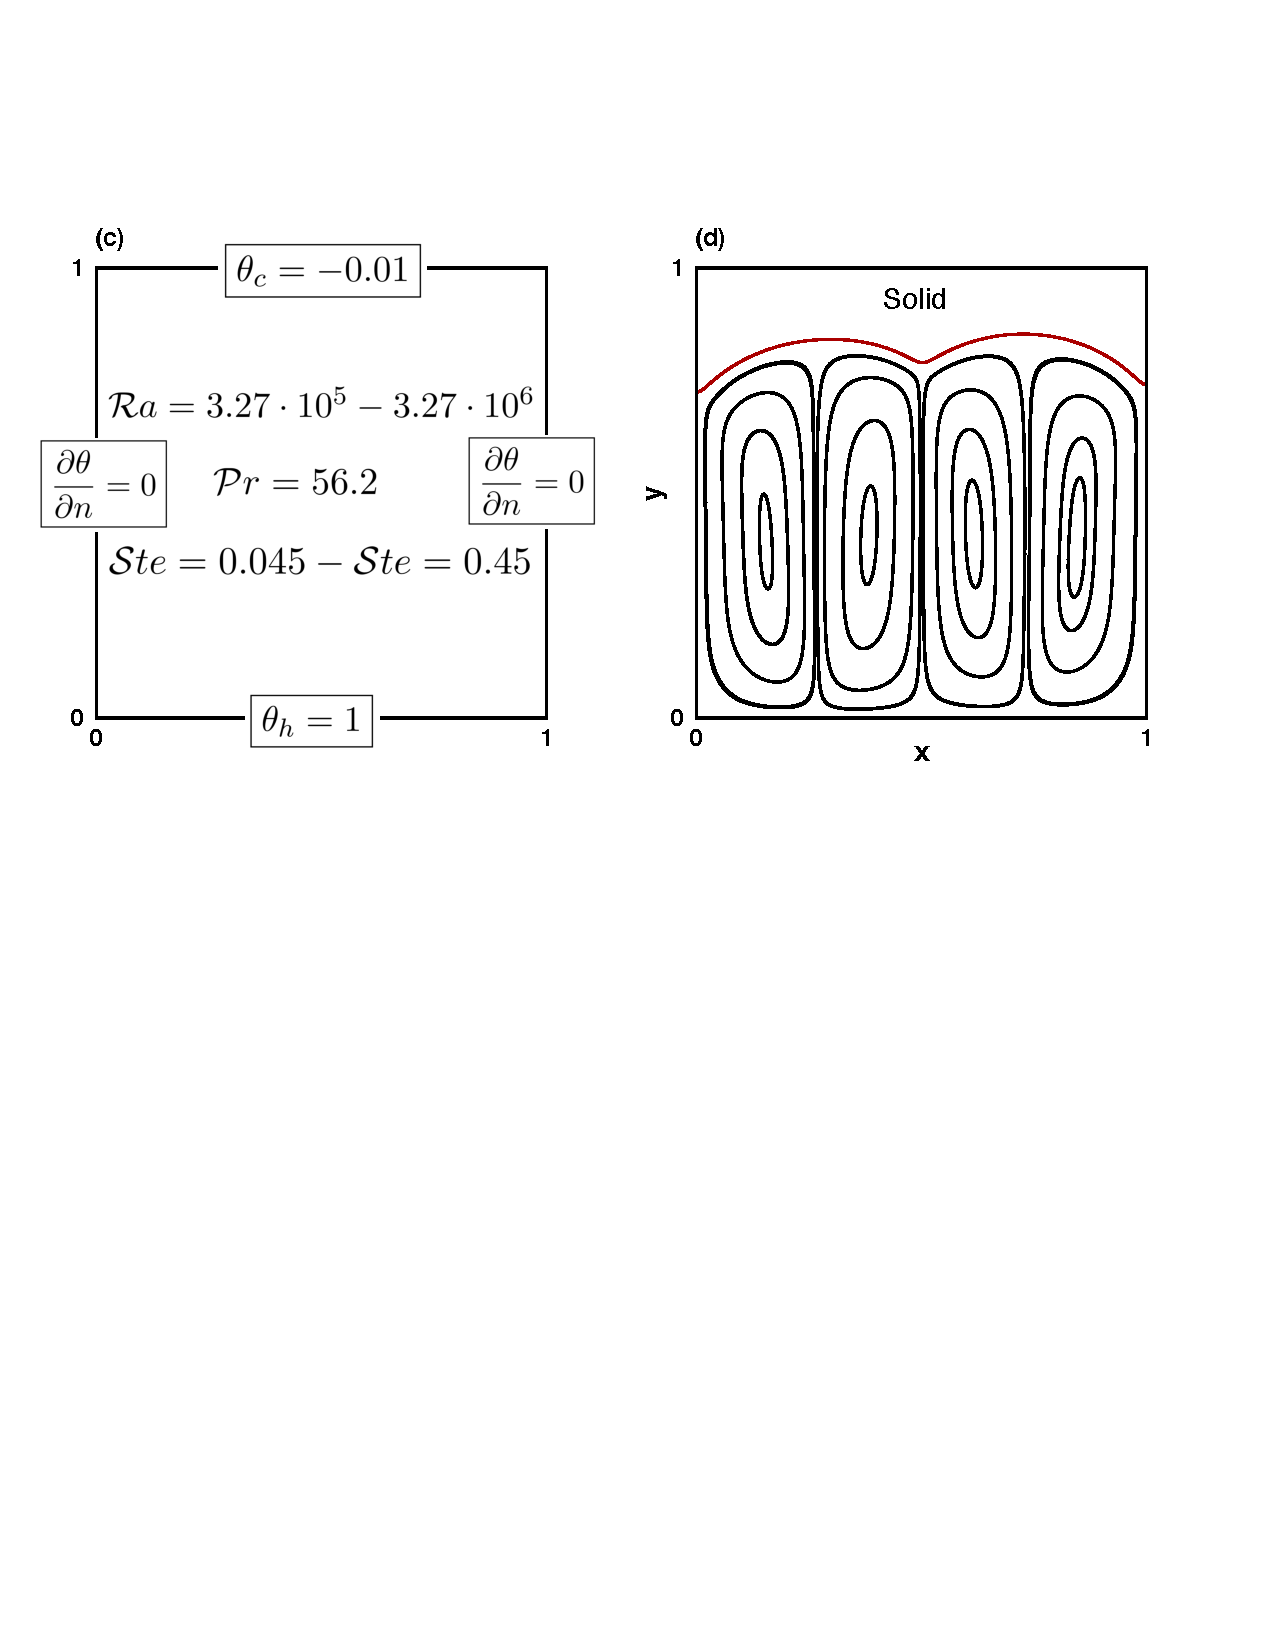
\includegraphics[width=\textwidth]{\figpath/Fig_cap_melting_basal/Scheme-melt-basal}
	\end{center}
	\caption{a.} \label{fig:melt-scheme}
\end{figure}
After the validation of the developed numerical method, the code is used as an investigation tool to analyse the phase-change process during the melting stage.
We consider a square cavity of height $H$ filled with n-octadecane and pay a closer attention to the temporal evolution of different physical parameter of the system. %, during the melting phase.
Two classes of convective melting system will be considered in this chapter: melting induced by lateral and basal heatings.
The dynamic of the melting is actually known to be fundamentally different for each of the two cases.
The shape of the interface and the streamlines in the fully developed convective flow are illustrated in panels (b) and (d) of Fig. (\ref{fig:melt-scheme}) for both cases.

The melting of PCM heated from the side could be representative of buildings applications, at the example of Fig. (\ref{fig:expe-PCM_Gong}) in which a brick of PCM is used as smart material to control the indoor environment of a building.
\cite{barreneche2016situ} have shown that wall made of PCMs allows to reduce the temperature peak about $20 \%$.
Bricks made of PCM melt from temperature difference between outdoor and indoor temperature differences and store the energy in the form of latent heat.
Other applications such as solar collectors or other thermal energy storages are also typical of such configurations.
In any cases, accurate assessment of the heat transfer is always essential.
Analytical investigation of \cite{bejan1989analysis} and scaling analysis of \cite{jany1988scaling} have permitted to describe the heat transfer during the melting by the mean of $N\!u$-$\Ray$ correlation.

The second class refers to passive temperature control for electronic devices or for geophysical problems such as lava lakes \citep{davaille1993thermal}, thermal convection in magma chambers \citep{brandeis1989convective} or ice-melt lakes \citep{polashenski2012mechanisms}. Ice-melt ponds that form during summer season in the Arctic \citep{polashenski2012mechanisms,esfahani2018basal} are known for example to display natural convection coupled to a phase-change process on the bottom side. In that case, Rayleigh-B�nard like convection cells are observed in the liquid phase.
Experimental \citep{hale1980solid,diaz1984visualization} and numerical \citep{esfahani2018basal,madruga2018dynamic,favier2019rayleigh} analysis of the dynamic of melting could be find in the literature.
Notwithstanding linear and weakly non-linear instability analysis based on a vanishingly small Stefan number assumption \citep{vasil2011dynamic}, no purely theoretical description of the heat transfer was investigated.
Some comparisons with theories \citep{malkus1954heat,grossmann2000scaling} made in the frame of Rayleigh-B�nard convection flow have been however carried out \citep{esfahani2018basal,madruga2018dynamic,favier2019rayleigh}.

Numerical comparison of the melting of n-octadecane with either lateral or basal heating is investigated in this chapter.
Mainly a comparison of the heat transfer involving in each case is of major interest.
Analysis of the time evolution of the lateral melting process followed by a scale analysis is presented first in Sec. \ref{sec-melting-lateral}.
The numerical results for the basal melting are given in Sec. \ref{sec-melting-basal}.

%\section{Boundary layer approximation and scale analysis} \label{sec-bound-scal-anal}
%Either PCM is used for energy storage or for building insulation or for other purposes, one would necessarily assess the heat transfer during the phase-change process.
%Mainly, it was extensively proven that the convective heat transfer plays significant role during the melting stage.
%Therefore, before solving numerically eqs. (\ref{eq-qmvt}) - (\ref{eq-energ}), we first rely on scale analysis to predict theoretically the fluid flow and heat transfer patterns that can develop in the fluid part.
%The idea behind the scaling analysis is about identifying the proper scales of the phenomenon, in order to understand the evolution of the heat transfer and the melting rates.
%
%In the present analysis, we will consider first only the liquid phase without phase-change.
%A further analysis of the scale during the melting will be developed in sec. (\ref{chap-MELTING-CAVITY}).
%We consider a two-dimensional enclosure of height H filled with Newtonian fluid, differentially heated from the vertical walls and insulated from the horizontal walls.
%A No-slip boundary condition is considered for the velocity. 
%Since no external force is applied to our system, the fluid flow is merely driven by natural convection flow, induced by temperature differences from the vertical walls.
%It is well-known from the foregoing boundary conditions that the fluid layer situated close to the vertical walls stuck to the wall and are motionless.
%The heat transfer through the fluid layer immediately adjacent to the wall is accordingly by pure conduction, i.e, $ q = - \left. (\partial \theta/ \partial x) \right |_{x=0} $.
%We therefore define the average Nusselt number to quantify the heat transfer rate at the heated wall:
%\begin{equation}\label{eq-def-Nu}
%   N\!u = - \int_0^1 \left. \frac{\partial \theta}{\partial x} \right |_{x=0} dy.
%\end{equation}
%
%When a steady state could be reached, the fluid near each sidewall is characterized by two boundary layers: a thermal boundary layer of thickness $\delta_{\theta}$ and a viscous boundary layer of thickness $\delta_\nu$.
%The boundary layer approximation assumes that the flow and the energy transfer are restricted predominantly to the boundary layer region.
%This theory was proposed first by Prandtl in 1904 and validated later by many experimental and numerical studies.
%The main consequences of the boundary layer approximations are that: \\
%{\it (i)} the normal part of the momentum equation has a negligible importance, \\
%{\it (ii)} the downstream diffusion term in the momentum and energy equations are neglected in comparison with the normal diffusion terms ($\partial^2 \vec{u}/\partial y^2 \ll \partial^2 \vec{u}/\partial x^2$ and $\partial^2 T/\partial y^2 \ll \partial^2 T/\partial x^2$) since the boundary layer thickness is much smaller than the enclosure height ($ \delta \ll H$), \\
%{\it (iii)} the pressure distribution is purely hydrostatic, i.e, $P = - \rho g y$, \\
%{\it (iv)} the thermal and the viscous boundary layer thickness are given by the order of magnitude expressions: $\delta_\nu/\delta_\theta = o \left(\Pr^{1/2} \right)$.\\
%These assumptions lead to the following boundary layer equations for the conservation of mass, momentum and energy:
%\begin{eqnarray} \label{eq-bound-mass}
%	\frac{\partial u}{\partial x} + \frac{\partial v}{\partial y} &=& 0, \\  \label{eq-bound-mom}
%	u \frac{\partial v}{\partial x} + v \frac{\partial v}{\partial y} &=& \nu \frac{\partial^2 v}{\partial x^2} + g \beta (T - T_{ref}), \\ \label{eq-bound-energy}
%	u \frac{\partial T}{\partial x} + v \frac{\partial T}{\partial y} &=& \alpha \frac{\partial^2 T}{\partial x^2}. 
%\end{eqnarray}
%The mass conservation in eq. (\ref{eq-bound-mass}) in the boundary layer region leads to:
%\begin{equation}
%	\frac{u}{\delta_\theta} \sim \frac{v}{H}.
%\end{equation}
%The energy eq. (\ref{eq-bound-energy}) expresses a balance between longitudinal convection and transverse conduction:
%\begin{equation}
%	\frac{v}{H} \sim \frac{\alpha}{\delta_\theta^2},
%\end{equation}
%which yields:
%\begin{equation} \label{eq-scale-v}
%	v \sim \frac{\alpha H}{\delta_\theta^2}.
%\end{equation}
%As far as momentum eq. (\ref{eq-bound-mom}) is concerned, we could identify the interplay among three forces:
%\begin{equation} \label{eq-scale-momentum}
%	\underbrace{\frac{v^2}{H}}_{inertia} \quad \underbrace{\nu \frac{v}{\delta_\theta^2}}_{friction} \quad \underbrace{g \beta \delta T}_{buoyancy}.
%\end{equation}
%Using the expression of $v$ in eq. (\ref{eq-scale-v}) and by dividing eq. (\ref{eq-scale-momentum}) by $g \beta \delta T$, we obtain:
%\begin{equation} \label{eq-final-scale}
%	\underbrace{\left( \frac{H}{\delta_\theta} \right)^4 Pr ^{-1} \Ray^{-1}}_{inertia} \quad  \underbrace{\left( \frac{H}{\delta_\theta} \right)^4 \Ray^{-1}}_{friction} \quad \underbrace{1}_{buoyancy}.
%\end{equation}
%Eq. (\ref{eq-final-scale}) indicates that the behaviour of the fluid in the boundary layer depends on the $\Pr$ number. \\
%First, for a high-Prandtl fluid ($\Pr \geq 1$), the friction-buoyancy balance yields: 
%\begin{equation} \label{eq-scale-nbd-high-Pr}
%	\delta_\theta \sim H \Ray^{-1/4}.
%\end{equation}
%The Nusselt number from eq. (\ref{eq-def-Nu}) scales as $H/\delta_\theta$, resulting: 
%\begin{equation}
%	N\!u \sim Ra^{1/4}
%\end{equation}
%and $v \sim \alpha/H \Ray^{1/2}$. \\
%Second, for a low-Prandtl fluid ($\Pr \ll 1$), we observe a balance between inertia and buoyancy, leading to:
%\begin{equation} \label{eq-corr-Low-Pr}
%	\delta_\theta \sim H Pr^{-1/4} \Ray^{-1/4}.
%\end{equation}
%Accordingly we obtain a Nu-Ra correlation:
%\begin{equation}
%	Nu \sim Pr^{1/4} \Ray^{1/4}.
%\end{equation}
%
%
\section{Melting of n-octadecane PCM with lateral heating}  \label{sec-melting-lateral}
%\subsection{Analysis of the time evolution of the melting process}
We consider the physical properties of n-octadecane given in Tab. (\ref{tab-param-PCM}) and investigate different height $H$ of the cavity and different value of $\delta T$ to assess the influence of the $\Ray$ number.
The numerical configuration is sketched in Fig. (\ref{fig:melt-scheme}a).
$\Ray$ numbers ranging from $3.27 \cdot 10^5$ to $6.54 \cdot 10^6$ are investigated.
For the $\Ray$ and $\Ste$ considered, the assumption of $(\beta \times \delta T) \ll 0.01$ is verified.

\subsection{Analysis of the time evolution of the melting process} \label{subsec-time-evol-lat}

We start by describing the time evolution of the melting process for the lower value of the $\Ste$ number.
We are interested in a slowly melting of the PCM to capture the transitions between the regimes described by \cite{jany1988scaling}, mainly the onset of the convective regime.
At $\tau=0$, the material is solid and the initial temperature is set to $\theta_0=-0.01$ everywhere inside the cavity. 
Then, the temperature of the left wall is suddenly increased to $\theta_h=1$, while the right wall is maintained at the same cold temperature $\theta_c=-0.01$. 
The material starts to melt, with a melting (identified by the iso-line $\theta=\theta_f=0$) propagating from the left to the right side of the domain. 
%The shape of the interface and the streamlines of the flow developing in the liquid phase when the convective flow is fully developped at $\tau = 0.06$ are illustrated in Fig. (\ref{fig:melt-scheme}b).
\begin{figure}
	\begin{center}
		%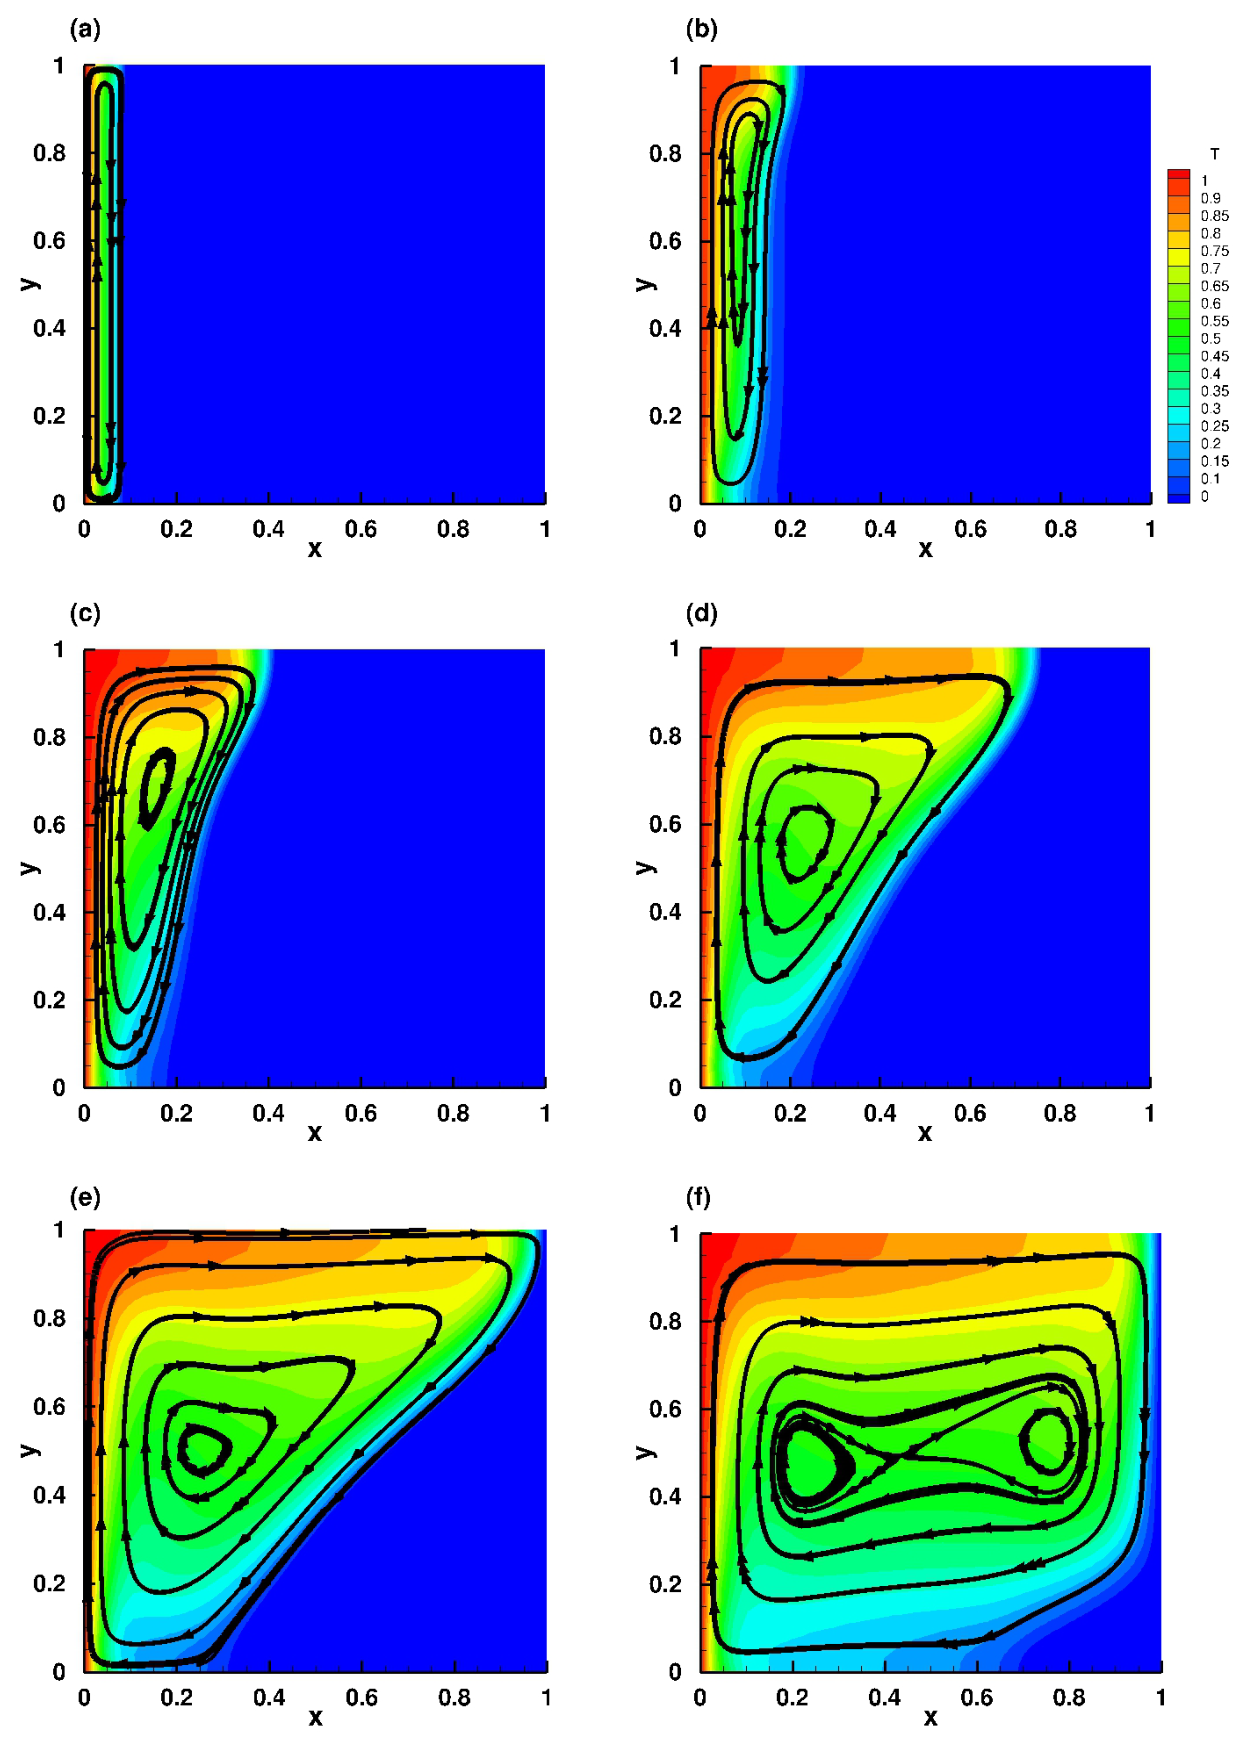
\includegraphics[width=.9\textwidth]{\figpath/Fig_cap_melting/fig05}
		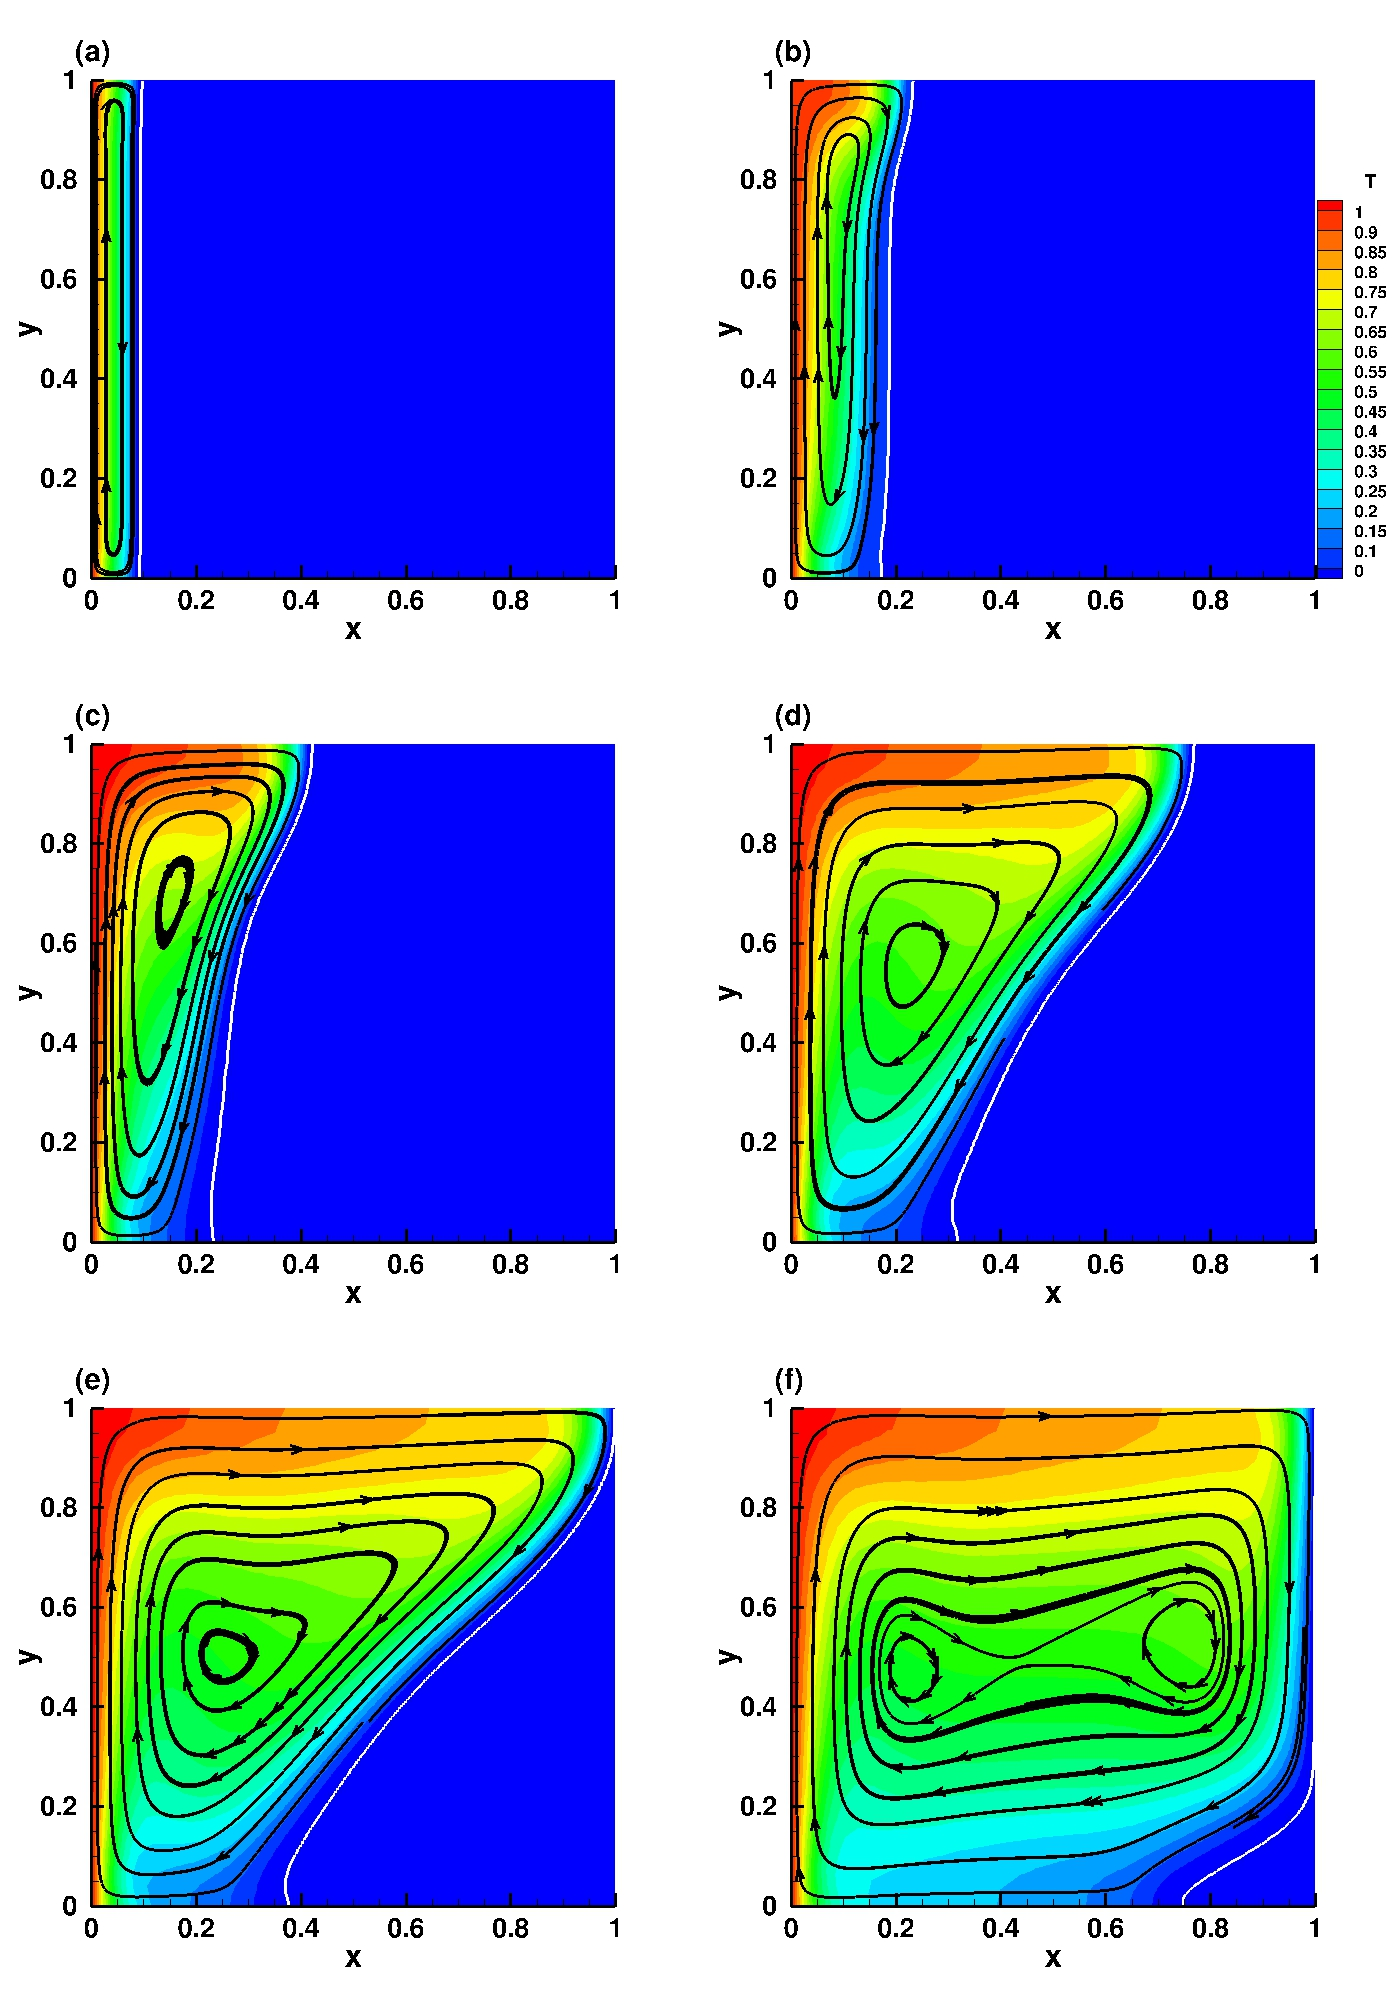
\includegraphics[width=\textwidth]{\figpath/Fig_cap_melting_basal/MELT_cavity_field}
	\end{center}
	\caption{Temperature iso-lines and streamlines in the fluid phase. The solid part is represented in blue and corresponds to the region of temperature $\theta \leq \theta_f=0$. Time instants (panels  a to f): $\tau=0.004; 0.016; 0.032; 0.063; 0.08; 0.2$. $\Ray = 3.27 \cdot 10^5$, $\Pr = 56.2$ and $\Ste = 0.045$.
		}\label{fig:melt-field}
\end{figure}

The time evolution of the phase-change system is depicted in Fig. \ref{fig:melt-field} for representative time instants.
Panels (a) to (f) offer the streamline showing the clockwise recirculation of the fluid, the melting front, and the temperature distribution (the solid phase is denoted by the blue region) for a comprehensive description of the evolution of the system. 
We can easily identify three different regimes describing the time evolution of the melting process. 
\begin{itemize}
	\item From $\tau=0$ to $\tau =0.004$ (Fig.  \ref{fig:melt-field}a), we note the vertical shape of the melting front, well predicted by the classical conduction model of \cite{stefan1891theorie}. This indicates that, at this stage, heat transfer is dominated solely by conduction.
	
	 \item Between $\tau =0.016$ to $\tau =0.032$ (Fig.  \ref{fig:melt-field}b), the natural convection in the fluid phase starts to alter the shape of the melting front.
	A mixed conduction and convection regimes rule the heat transfer. 	Convection mainly affects the upper part of the fluid motion, while conduction is still dominating in the lower part. As the volume thermal expansion coefficient $\beta$ is positive, we expect a clockwise circulation of the liquid inside the convection cell, as noted by \cite{jany1988scaling}.
	This also makes the liquid-solid interface to move faster at the top of the cavity, explaining the deformed shape of the melting front, which is a signature of the convection effects  (see also \cite{kowalewski2004phase}). 
	
	\item After $\tau=0.032$ (Fig.  \ref{fig:melt-field}c-d), natural convection dominates the heat transfer process and impacts radically the solid-liquid interface shape and motion.
	The melting front line exhibits four distinct regions characterized by different slopes with respect to the vertical axis. The largest slope is observed at the top of the cavity and is related to the particular shape of the convection cell. Note that top and bottom parts of the interface are normal to the cavity boundaries because of the imposed adiabatic boundary conditions.

	\item After $\tau =0.08$  the melting front is nearly touching the right wall of the cavity, firstly at the top (Fig.  \ref{fig:melt-field}e) of the cavity. The melting process continues and the fluid progressively fills the cavity, with a melting front  deforming to a vertical line. The  simulation of the melting process is stopped at $\tau =0.2$ (Fig.  \ref{fig:melt-field}f), when it is numerically difficult to separate the melting front from the right wall boundary. At this time instant,  the fluid fraction reaches the value of $0.95$ and  the melting of the PCM is considered to be complete, even though a small region of solid PCM remains at the lower right bottom of the cavity. Note from Fig.  \ref{fig:melt-field}f the existence in the fluid  of two recirculating zones instead of a single one observed during previous stages.
	
\end{itemize}

\subsection{Scale analysis of the melting} \label{sec:scaling anal}

We further analyse each of the three regimes cited previously and identify the proper scales proper of the phenomenon.
The following analysis is similar to that outlined in Sec. (\ref{sec-bound-scal-anal}) for natural convection problem without phase-change.
The location of the interface will be denoted by $\Gamma_i$.
At the solid-liquid interface, the energy balance condition which takes into account the released latent heat and the discontinuity of heat flux between the solid and the liquid can be handle by the following Stefan condition:
%\begin{eqnarray} \label{eq:Ste-condition}
%	\left. T\right|_{x=\Gamma_i} &=& T_f, \\ \nonumber
%	\rho h_{sl} \frac{\partial \Gamma_i}{\partial n} &=& - k \frac{\partial T}{\partial n},
%\end{eqnarray}
\begin{eqnarray} \label{eq:Ste-condition}
	\left. \theta \right|_{x=\Gamma_i} &=& \theta_f =  0, \\ \nonumber
	\frac{\partial \Gamma_i}{\partial n} &=& - \frac{\Ste}{\Prd} \frac{\partial \theta}{\partial n},
\end{eqnarray}

Immediately after $t=0$ (see Fig. (\ref{fig:melt-field}a)), the melted PCM occupy a thin enclosure of height $H$ and width $\Gamma_i$, with $\Gamma_i \ll H$ (and thus $\partial^2 \theta/\partial y^2 \ll \partial^2 \theta/\partial x^2$).
In such configuration, the temperature varies linearly between the two sidewalls and the heat transfer is essentially ruled by conduction. 
The fluid phase is motionless and the horizontal heat flux across the incipient melting PCM is balanced by the enthalpy absorbed at the interface.
Accordingly, the interface remain vertical during this stage.

Since the velocity in the liquid phase is relatively small during this conductive regime, the momentum, the energy equations and the Stefan condition at the interface could be rewritten as follows in the small enclosure containing the melted PCM:
\begin{eqnarray} \label{eq-balance-momentum}
   \frac{\partial p}{\partial x} &=& \frac{\Ray}{\Rey^2 \Pr} \theta, \\ \label{eq-energy-x}
    \frac{\partial \theta}{\partial t} &=&  \frac{\partial^2 \theta}{\partial x^2}, \\ \label{eq-stefan-x}
   \frac{\partial \Gamma_i}{\partial t} &=& - \frac{\Ste}{\Prd} \frac{\partial \theta}{\partial x}.
\end{eqnarray}
The temperature field during the conduction regime is quasi-steady, thus linear eq. (\ref{eq-stefan-x}) can be approximated by:
\begin{equation}
    \frac{\partial \Gamma_i}{\partial t} \approx - \frac{\Ste}{\Prd} \frac{\theta_f - \theta_h}{\Gamma_i} \approx  \frac{\Ste}{\Prd} \frac{1}{\Gamma_i}.
\end{equation}
The location $\Gamma_i$ of the interface could hence be approximated by:
\begin{equation}
   \Gamma_i = \sqrt{2 \times \frac{\Ste}{\Prd} t} = \sqrt{2 \tau}.
\end{equation}
Moreover, the Nusselt number can be evaluated using the same assumption:
\begin{equation}
   N\!u= \int_0^{1} \left. \frac{\partial \theta}{\partial x} \right|_{x=0} dy \approx \frac{1}{\Gamma_i} \approx ({2 \tau})^{-1/2}.
\end{equation}
To summarize, during the first stage of the melting, when the heat transfert is lead by conduction, the time evolution of the liquid fraction (given by the location of the interface) and the Nusselt number can be approximated by
$L_f \sim \tau^{1/2}$ and $N\!u \sim \tau^{-1/2}$.

\begin{figure}
	\begin{center}
		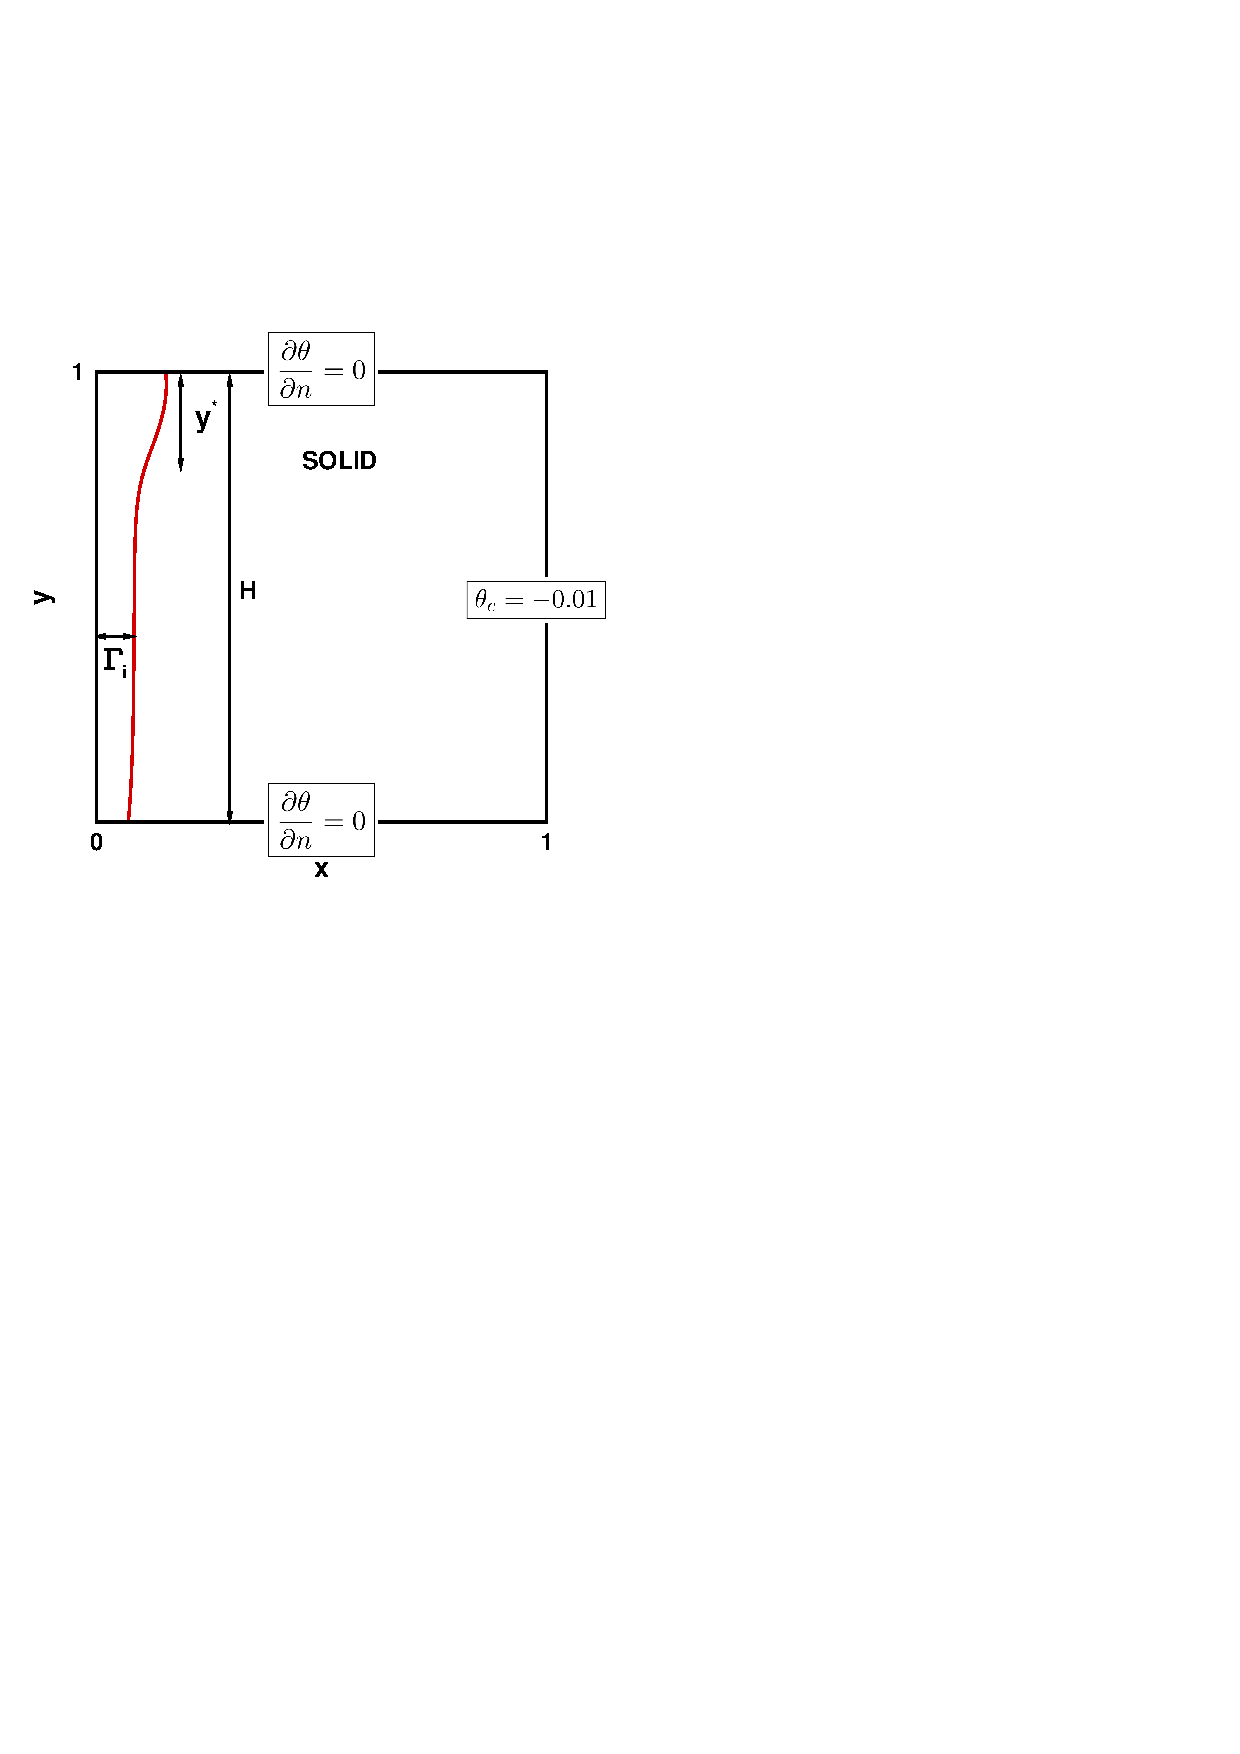
\includegraphics[width=.5\textwidth]{\figpath/Fig_cap_melting_basal/MELT_Regime_evol}
	\end{center}
	\caption{Illustration of the mixed regime. Solid red line is the solid-liquid interface, $\Gamma_i$ represents the location of the interface and $y^*$ denote the height of fluid impacted by the emerging convective flow.}\label{fig:melt-scheme-regime}
\end{figure}


While the melting continue to expand to the right side of the domain, a natural convection flow emerges from the top of the cavity (see Fig. (\ref{fig:melt-scheme-regime})).
Convection and conduction coexist at this stage. 
The total heat transfer rate is the sum of the conductive and the convective heat transfer.
Turning back to the energy eq. (\ref{eq-energ}), a competition among three distinct effects could be identified:
\begin{equation}
	\underbrace{\frac{\Delta \theta}{t}}_{Inertia} \quad \underbrace{v \frac{\Delta \theta}{H}}_{Convection} \quad \underbrace{\alpha \frac{\Delta \theta}{\Gamma_i^2}}_{Conduction},
\end{equation}
As $t$ increases, the inertia decreases in importance, the convection effet increases since it is proportional to $v$ and the conduction becomes more and more negligible because $\Gamma_i$ is increasing with time. 
To assess for the convective heat transfer contribution during this mixed regime,
one can define a Rayleigh number based on $y^*$ as $\Ray_{y^*} = \Ray \times y^{*3}$,
with $y^{*}$ the height of the liquid zone altered by the convection flow as shown in Fig. (\ref{fig:melt-scheme-regime}).
We note that at the bottom part of the cavity, the interface remains vertical by the effect of the conductive heat transfer (see Fig.).
Since $\Pr \gg 1$, the scaling presented in eq. (\ref{eq-scale-nbd-high-Pr}) allows to evaluate the thermal boundary layer in the top region as:
 \begin{equation} \label{eq-conv-cond-reg}
 \delta_{\theta}^* \sim y^* \times \Ray_{y^*} ^{-1/4}.
\end{equation}
A this stage, the thickness $\delta_{\theta}^*$ of the thermal boundary layer is proportional to the thickness $\Gamma_i$ ($\sim \tau^{1/2}$) resulting that:
 \begin{equation}
	 y^* \sim (2 \tau)^2 \times \Ray \quad \Rightarrow \quad \frac{y^*}{\Gamma_i} \sim (2 \tau)^{3/2} \times Ra. .
 \end{equation}
The Nusselt number during the mixed convection-convection regime can therefore be approximated by:
\begin{equation} \label{eq-Nu-conv-cond}
   N\!u \sim (2 \tau)^{-1/2} + (2 \tau)^{3/2} \times \Ray
\end{equation}
Eq. \ref{eq-Nu-conv-cond} indicates that the contribution of the conduction ($(2 \tau)^{-1/2}$) decreases with time while the convection one is increasing.
%From a simple analysis of $\partial N\!u/\partial \theta = 0$, one can find the minimum value of the Nusselt number $N\!u_{min} \sim Ra^{1/4}$ occurring at $\tau \sim \Ray^{-1/2}$.

Finally, when the natural convection flow is fully developed and dominates the heat transfer along the vertical heated wall the thermal boundary layer is $\delta_T \sim Ra^{1/4}$ and therefore the Nusselt number scale is:
\begin{equation}
   N\!u \sim Ra^{1/4}
\end{equation}

\cite{Okada1984} have suggested from their experimental data the following correlation of $N\!u$ taking into account the foregoing presented regimes:
\begin{equation} \label{eq-corr-Okada}
	N\!u = \left \{
	      %\begin{array}{ll}
	      \begin{aligned}
	      		\frac{1}{\sqrt{2 \tau}} \quad  &\text{if} \quad \tau \leq \tau_t, \\ 
	      		\frac{1}{\sqrt{2 \tau_t}} \left \{ 1 + C (\tau - \tau_t) \right \} \quad & \text{if} \quad \tau > \tau_t, \\
			c_1 \Ray^{0.266} \quad & \text{otherwise},
	       %\end{array}  
	       \end{aligned}
	\right.
\end{equation}
with $c_1 = 0.234$ a constant fitted from the experimental data, $\tau_t$ the transition time from conduction to convection.
\cite{jany1988scaling} have proposed the following single correlation, also combining the regimes described previously:
\begin{equation} \label{eq-Nu-scale}
N\!u(\tau) =  \frac{1}{\sqrt{2 \tau}} + \left[c_1 \Ray^{1/4} - \frac{1}{\sqrt{2 \tau}} \right]  \left[ 1 + \left(c_2 \Ray^{3/4}  \tau^{3/2}\right)^n \right]^{1/n}.
\end{equation}
The values of the constants were fitted from numerical data: $c_1 = 0.27$, $c_2 = 0.0275$, and $n=-2$. 

Both of eqs. (\ref{eq-corr-Okada}) and (\ref{eq-Nu-scale}) are compared with our numerical results in Fig. (\ref{fig:Nusselt}) showing the time evolution of the Nusselt number at the left wall.
%In Fig. \ref{fig:Nusselt} we compare the time evolution of the Nusselt number obtained from our numerical data (see Figure \ref{fig: pcm-case})  to experimental results of  \cite{Okada1984}  and predictions obtained from the correlation (\ref{eq-Nu-scale}). 
Our results perfectly fit with the theoretical prediction of \cite{jany1988scaling} and are also in good agreement with the correlation of \cite{Okada1984}. %, suggesting, however, that very accurate measurements and numerical simulations are needed to validate theoretical scaling analysis.
The gap between the current simulation and the results of \cite{Okada1984} could be explained by the experimental heat loss mentioned by the author and the uncertainties of the experimental measurements.
The regimes described by the shape of the interface in Sec. (\ref{subsec-time-evol-lat}) could be featured by the temporal evolution of $N\!u$:
\begin{enumerate}
	\item The pure conduction regime ($N\!u \sim (2 \tau)^{-1/2}$) for $\tau  \gtrsim 0$ to $\tau \sim \Ray^{-1/2} =0.02$  (corresponding to Fig.  \ref{fig:melt-field}a).
	Since the temperature gradient has initially huge values because of the sudden increase of the temperature of the left wall, the Nusselt number rapidly decreases during the first stage of the flow evolution. 
	The  signature of this conduction regime is the slow heat transfer characterized by a monotonic decrease of the Nusselt number.
	
	\item The mixed conduction-convection regime  ($ N\!u \sim \tau^{-1/2} + \Ray\, \tau^{3/2}$) for $  0.02  \leq \tau \leq 0.05$ (illustrated in  Fig.  \ref{fig:melt-field}b).

	\item The convection dominated regime ($ N\!u \sim \Ray^{1/4}$) for $\tau > Ra^{-1/2}$  (corresponding to Figs.  \ref{fig:melt-field}c-e).
	The plateau at the value of $\Ray^{1/4}$ corresponds to the pure convective transfer and is observed in Fig. \ref{fig:Nusselt} for $  0.05 \leq \tau \leq 0.1$. Numerical results show a slight decrease of the $N\!u$ in the final stage ($\tau \geq 0.1$), when the melting front starts to touch the right wall of the cavity (see Figs.  \ref{fig:melt-field}e-f). The correlation model is not valid for this late evolution of the melting process.
\end{enumerate}

\begin{figure}
	\begin{center}
		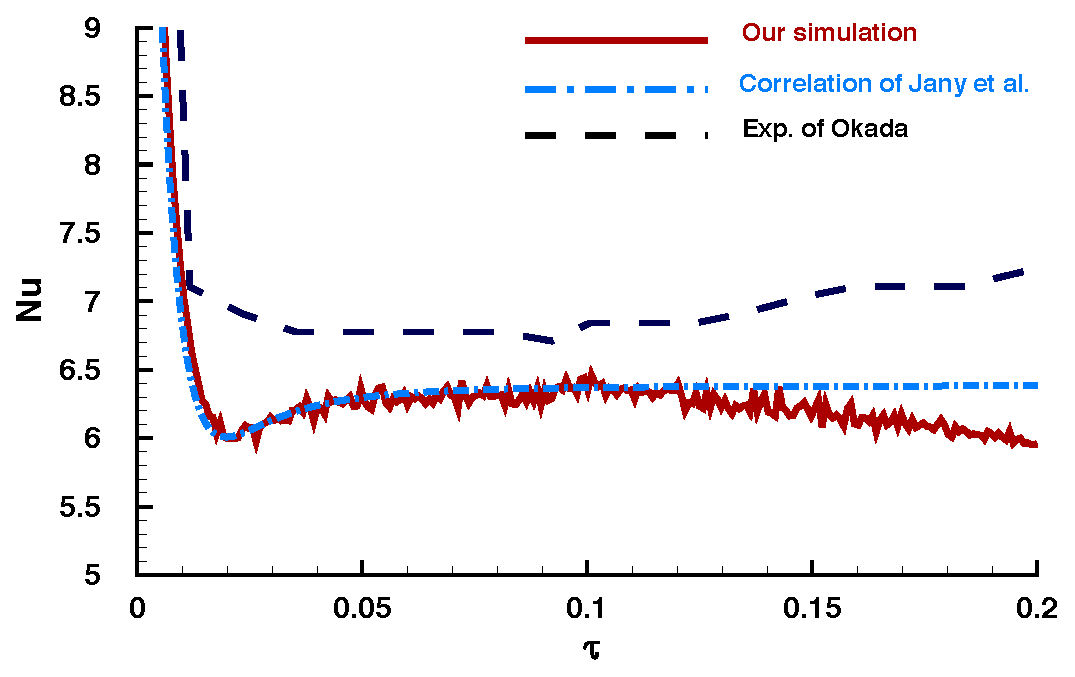
\includegraphics[width=.7\textwidth]{\figpath/Fig_cap_melting/fig06}		
	\end{center}
	\caption{Complete melting of the PCM. Time evolution of the average Nusselt number defined at the hot (left) wall (cf. eq. \ref{eq-def-Nu}) (solid line). Comparison with the experimental results of  \cite{Okada1984} (dashed line) and the predictions using the correlation (\ref{eq-Nu-scale}) suggested by \cite{jany1988scaling} (dash-dot line). $\Ray = 3.27 \cdot 10^5$, $\Pr = 56.2$ and $\Ste = 0.045$.}\label{fig:Nusselt}
\end{figure}


Another important basic quantity describing the melting process is the liquid fraction $L_f$.  
The time evolution of the liquid fraction (Fig. \ref{fig:Lf}a) displays three regimes during the melting process. $L_f$  initially grows as $\tau^{ 1/2}$, which is a typical law for a conduction-dominated heat transfer. Then, a linear temporal evolution is observed, until the melting front reaches the right wall.
This linear regime corresponds to the quasi-steady state observed in the evolution of the Nusselt number (Fig. \ref{fig:Nusselt}).

Using the asymptotic limits of Eq. (\ref{eq-Nu-scale}) for $ \tau \to 0$ (pure conduction) and $ \tau \to \infty$ (pure convection),  \cite{jany1988scaling} suggested the following correlation law for the time evolution of the liquid fraction:
\begin{equation} \label{eq-Lf-scale}
L_f(\tau) = \left[\left({\sqrt{2 \tau}} \right)^5 + \left(c_1 \Ray^{1/4}  \tau \right)^{5} \right]^{1/5},
\end{equation}
where $c_1=0.27$ is the same constant as in (\ref{eq-Nu-scale}). We compare in Fig. \ref{fig:Lf}b our numerical results with the predictions based on (\ref{eq-Lf-scale}) within the validity domain of the analysis, \ie before the melting front reaches the right wall of the cavity. A very good agreement is found with theoretical predictions and also with previously published numerical results \citep{Wang2010}.

\begin{figure}[!h]
	\begin{center}
		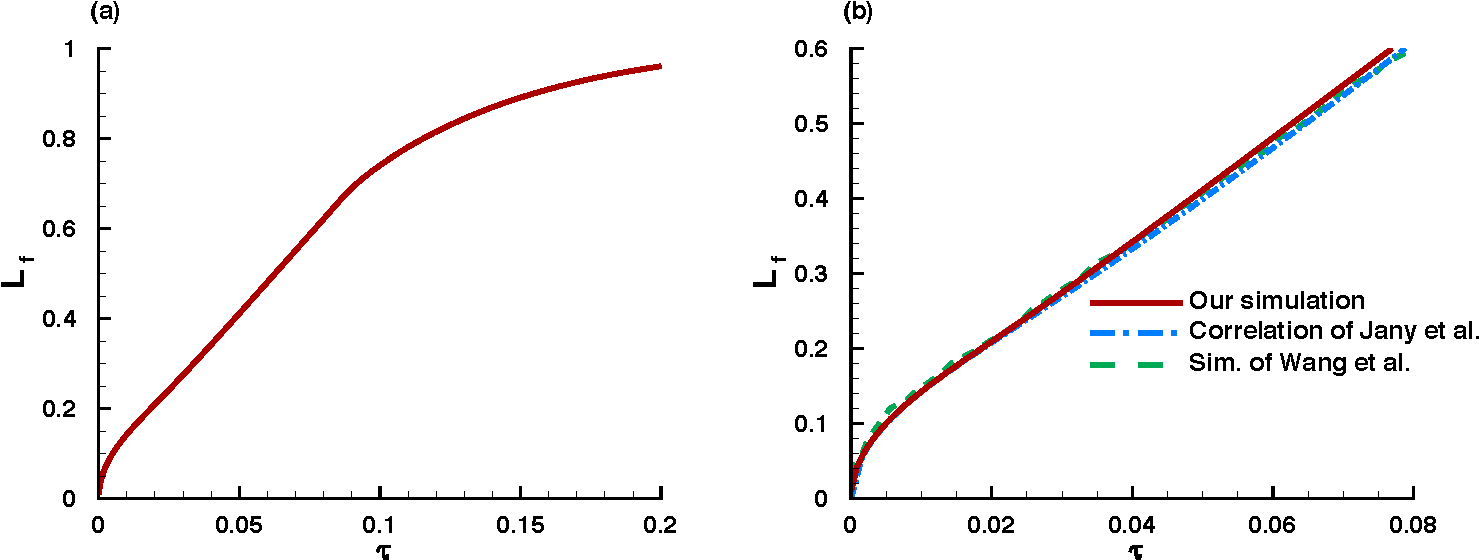
\includegraphics[width=0.9\textwidth]{\figpath/Fig_cap_melting/fig07}
	\end{center}
	\caption{Complete melting of the PCM. (a) Time evolution of the liquid fraction for the complete melting of the PCM. (b) Comparison of our results (solid line) with the numerical results of  \cite{Wang2010} (dashed line) and the predictions using the correlation (\ref{eq-Lf-scale}) suggested by \cite{jany1988scaling} (dash-dot line).}\label{fig:Lf}
\end{figure}


%%%%%%%%%%%%%%%%%%%%%ù
\subsection{Influence of the Rayleigh number}
%%%%%%%%%%%%%%%%%%%%%

\begin{figure}
	\begin{center}
		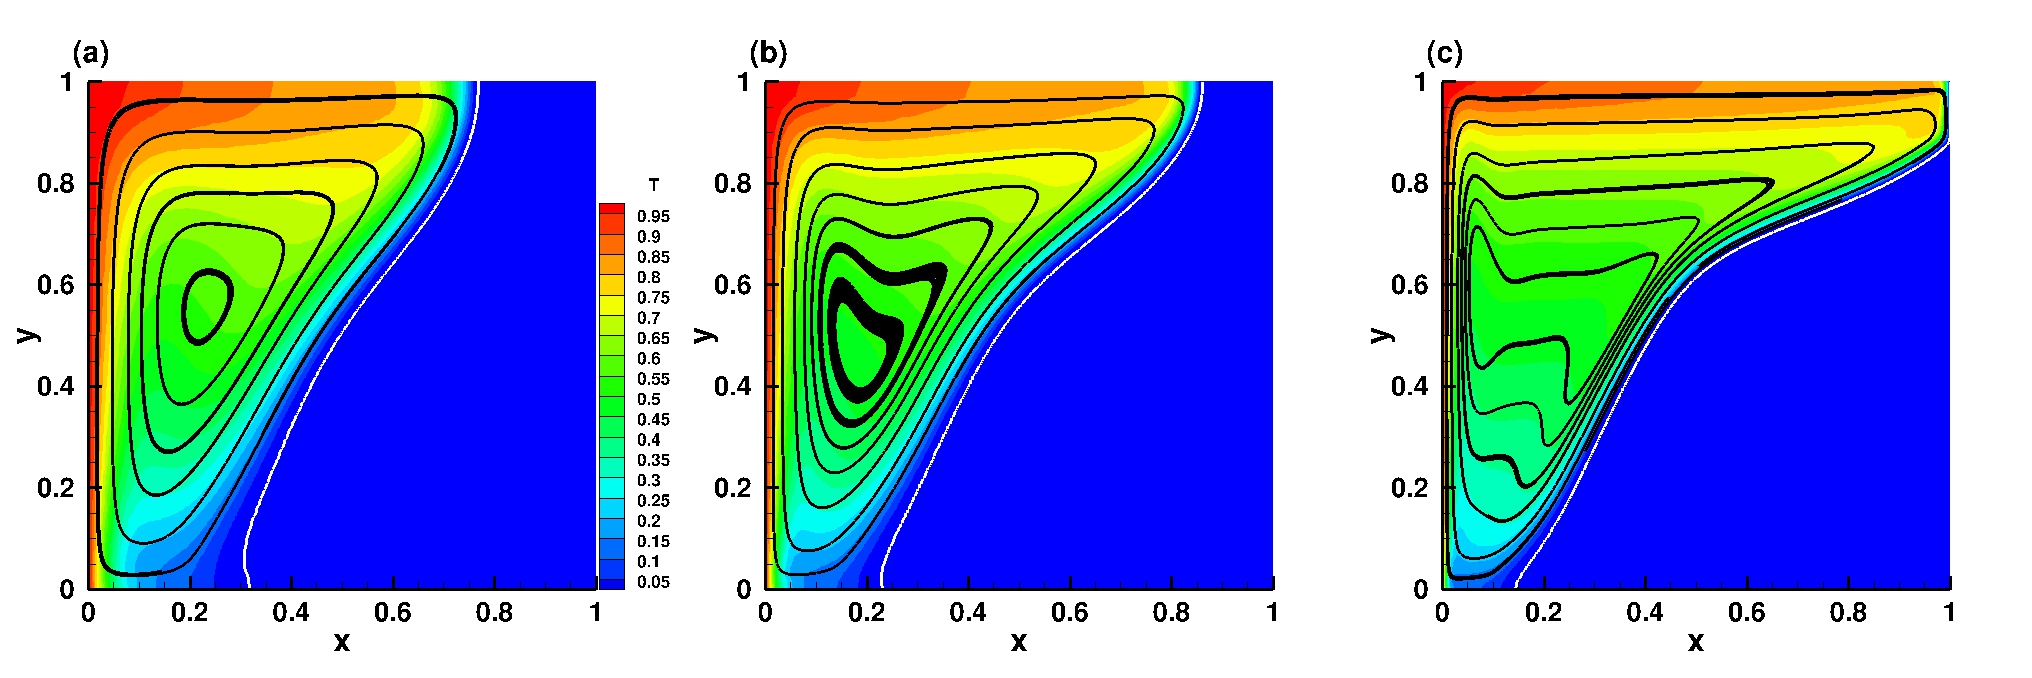
\includegraphics[width=\textwidth]{\figpath/Fig_cap_melting_basal/MELT_cavity_Ra_comp}
	\end{center}
	\caption{PCM melting at $L_f = 0.5$. Illustration of the temperature field, the streamlines, and the melting front for three $\Ray$ numbers: (a) $\Ray = 3.27 \cdot 10^5$ , (b) $\Ray = 1.62 \cdot 10^6$, (c) $\Ray = 3.27 \cdot 10^6$.
	The $\Prd$ and $\Ste$ numbers are kept constant: $\Prd = 56.2$ and $\Ste = 0.045$.} \label{fig:melt-comp-Ra}
\end{figure}

To investigate the influence of the Rayleigh number on the evolution of the melting process, we performed different simulations by multiplying the initial value of $\Ray = 3.27 \cdot 10^5$ by a factor of 5 and 10, respectively. The exact values are: $\Ray = 1.62 \cdot 10^6$ and $\Ray = 3.27 \cdot 10^6$. 
First, we increase the height $H$ of the cavity by a factor of $\sqrt[3]{5}$ and $\sqrt[3]{10}$ and consider the same $\delta T$.
Thus the Stefan number $\Ste$ is kept constant.
Second, we increase the temperature difference parameter $\delta T$ by keeping $H$ constant.
It corresponds of an increased value of the Stefan number by a factor of $5 $ and $10$:
$\Ste = 0.223$ and $\Ste = 0.45$.

Snapshots of numerical solutions for $\Ray = 3.27 \cdot 10^5$,  $\Ray = 1.62 \cdot 10^6$ and  $\Ray = 3.27 \cdot 10^6$ at constant $\Ste$ number are given in Fig. (\ref{fig:melt-comp-Ra}).
The colours correspond to the temperature distribution, the  black lines correspond to the streamlines and the white lines correspond to the solid-liquid interface.
Panels (a) to (c) denote the dynamic of the convective melting when half of the initial solid PCM ($L_f = 0.5$) have melted.
The top part of the interface moves faster while the bottom one is slowed by the increasing value of $\Ray$.
At constant $\Ste$ and $\Prd$ numbers, the interface velocity is proportional to $\partial T / \partial n$, which is maximum at the top of the cavity because of the clockwise recirculation of the fluid explaining the observed trends.

Figs \ref{fig:Ra-Nusselt-H} and \ref{fig:Ra-Nusselt-deltaT} show the temporal evolution of the liquid fraction $L_f$ (a),  and the average Nusselt number defined at the hot wall,  (b). 
The same heat transfer regimes described previously are observed for each case: conduction, mixed conduction-convection and convection.

Fig. \ref{fig:Ra-Nusselt-H}(a) indicates that increasing the Rayleigh number by keeping $\delta T$ constant induces a slower melting rate.
This is the expected behaviour since the size of the PCM is increased by a factor of 2, and the velocity $\vec u$ is hence decreasing  in order to satisfy the condition $\Rey = 1$.
We note however a non-monotonic variation of time necessary to melt a fixed value of fluid.
For instance, to achieve $L_f = 0.5$ (50\% of the volume is melted), an increase of $\Ray$ by a factor of $10$ leads to a growth of the time by a factor of $1.7$.
Nonetheless, when $\Ray$ is  $5$ times larger, the necessary time only increases by a factory of $2$.
This is most likely due to the non-linear intricacies of the problem and requires further investigation.
Furthermore, the Nusselt number reported in Fig. \ref{fig:Ra-Nusselt-H}(b) shows that the higher the Rayleigh number, the higher the Nusselt number.
This is consistent, since the temperature gradient is integrated along a greater heated wall. 

Fig. \ref{fig:Ra-Nusselt-deltaT}(a) shows that by increasing the value of $\delta T$ and consequently increasing the Rayleigh number and the Stefan number, the PCM melts faster. 
We note that the heigh $H$ of the cavity is kept constant, hence the natural convection flow in the melted PCM is enhanced when the Rayleigh number keep increasing.
As a consequence, the convection-dominated regime is reached earlier, as shown by the shift of the minimum of the $N\!u$ to lower values of $t_{\varphi}$ in Fig. \ref{fig:Ra-Nusselt-deltaT}(b). This evolution is also observed for the liquid fraction. 
As expected, an increase of the Rayleigh number and the Stefan number is followed by an enhancement of the heat transfer during the melting, and consequently an improved efficiency of the PCM.
\begin{figure}
	\begin{center}
		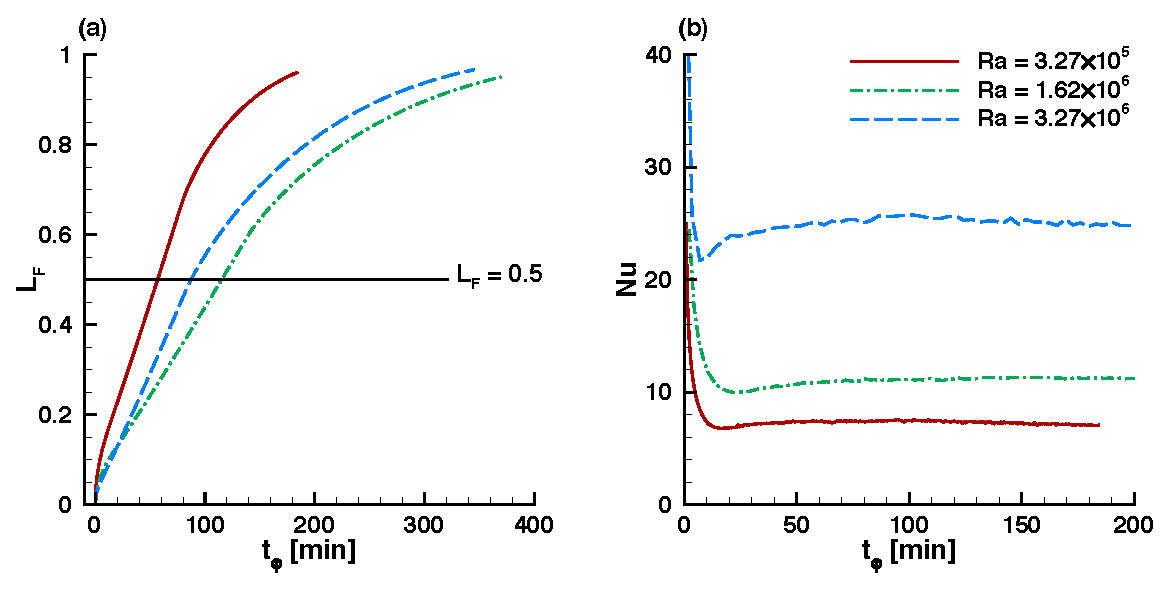
\includegraphics[width=\textwidth]{\figpath/Fig_cap_melting/fig08}
	\end{center}
	\caption{Complete melting of the PCM.  Influence of the value of the Rayleigh number ($\Ray$) on the time evolution of the average Nusselt number defined at the hot (left) wall (a) and liquid fraction (b). The reference case ($\Ray=3.27\cdot 10^5$) is represented by red continuous lines. The value of the $\Ray$ was increased by a factor of $5$ and $10$, respectively while the Stefan number $\Ste$ is kept constant.}\label{fig:Ra-Nusselt-H}
\end{figure}

\begin{figure}
	\begin{center}
		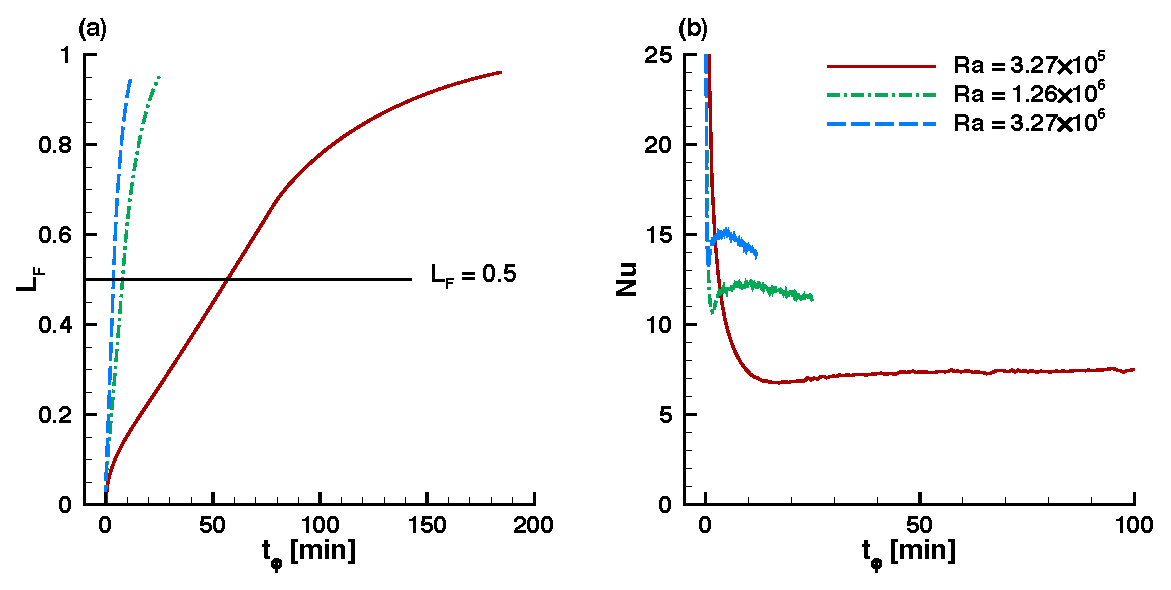
\includegraphics[width=\textwidth]{\figpath/Fig_cap_melting/fig09}
	\end{center}
	\caption{Complete melting of the PCM.  Influence of the value of the Rayleigh number ($\Ray$) on the time evolution of the average Nusselt number defined at the hot (left) wall (a) and liquid fraction (b). The reference case ($\Ray=3.27\cdot 10^5$) is represented by red continuous lines. The value of the $\Ray$ and $\Ste$ were increased by a factor of $5$ and $10$, respectively.}\label{fig:Ra-Nusselt-deltaT}
\end{figure}

\newpage
\clearpage
\section{Melting of octadecane PCM with basal melting} \label{sec-melting-basal}


The melting of PCM heated from the side was presented in Sec. \ref{chap-MELTING}.
The dynamic of the melting, the identification of three regimes describing the melting process and the effect of the Rayleigh number have been discussed in detail.
In this section, we pay more attention to PCM heated from below.
This configuration is indeed known to be overspread in the nature or in human activities, such as geophysical flows (Earth's mantle formation, magma oceans) or heat dissipation from electronic devices.

While the melting of PCM heated from the side have attracted many consideration, the melting of PCM heated from below have received less attention.
\cite{diaz1984visualization,hale1980solid} have studied experimentally the solid-liquid interface morphology of PCM during basal heating.
\cite{gong1998flow} studied numerically the flow and heat transfer during the melting of pure n-octadecane in a rectangular cavity heated from below.
Recent numerical simulations investigate different boundary conditions such as
periodic configurations along the horizontal axis \citep{esfahani2018basal,madruga2018dynamic,favier2019rayleigh} or wavy surface in a rectangular cavity heated from below \citep{kousksou2014melting}.

 We investigate in this chapter the melting of a pure octadecane PCM in a square enclosure heated from below.
 The dynamics of the melting is fundamentally different in the basal heating case compared with the lateral heating.
 It has been observed that for this configuration natural convection develops in the form of Benard cells and
 results in a nonplanar solid-liquid interface. 
\cite{vasil2011dynamic,favier2019rayleigh} have studied the hydrodynamic instabilities at the onset of convection and compared their observation with the classical Rayleigh-B�nard instability mechanism \citep{chandrasekhar2013hydrodynamic}.
\cite{favier2019rayleigh} have focused their attention to the effect of the non-planar topography of the interface to the convection flow.
 On the other hand, \cite{gong1998flow,esfahani2018basal,madruga2018dynamic} mostly focused on global quantities such as the heat flux and the statistical properties of the interface.

The physical parameters considered are the same as presented in Sec. \ref{sec: melting-2D}:
$\Pr = 56.2$ and $\Ste = 0.045$.
Three Rayleigh numbers are carried out: $\Ray = 3.27 \cdot 10^5$, $\Ray = 1.62 \cdot 10^6$, $\Ray = 3.27 \cdot 10^6$ to assess the influence of the size of the domain on the dynamic of the natural convection flow
as observed by \cite{madruga2018dynamic}.
The PCM is initially solid at a cold dimensionless temperature $\theta_c$ under the temperature of fusion.
The top of the wall is set at an isothermal temperature $\theta = \theta_c$, the vertical wall are adiabatic and the bottom is heated at a dimensionless temperature $\theta = \theta_h$.
 We investigate two-dimensional numerical simulation even if 
 \cite{gau1983flow} and  \cite{gong1998flow} have noticed the existence of three-dimensional convection cells during the very first step of the melting process.
 Indeed, this three-dimensional convection cell can be neglected since the duration is very short compared with the whole melting step,
so that the two-dimensional model is realistic.
A qualitative observation of the dynamic of the natural convection flow and its impact on the melting front is first addressed.
Second, the observation of four regimes during the melting is discussed.
Finally, a comparison between the lateral and the basal heating is given.

\subsection{Time evolution of the melting process} \label{sec-RB-melt-process}

The natural convection flow in the melt PCM during lateral heating exhibits convection cells deforming the solid-liquid interface (see Fig. \ref{fig:melt-field}).
The dynamic of the natural convection flow during the basal heating is fundamentally different.
It is well known that any non-planar topography can lead to a baroclinic flow at any Rayleigh number.

Fig. \ref{fig:melt-below} displays the structure of the natural convection in the melt PCM through a sequence of panels for temperature isolines and streamlines in the liquid phase.
An array of lengthening plumes (panel a to c) and counter-rotating convective cells (panel d to f)  is located in the liquid phase.
The number of convective cells and plumes increases with the Rayleigh number.
For $\Ray = 3.27 \cdot 10^5$, three equidistant plumes (Fig. \ref{fig:melt-below}a) and five convective cells (Fig. \ref{fig:melt-below}d) can be observed, while four and six plumes are observed for $\Ray = 1.62 \cdot 10^6$ and $\Ray = 3.27 \cdot 10^6$ respectively (Figs. \ref{fig:melt-below}b and \ref{fig:melt-below}c).
These observations agree well with the numerical results of \cite{gong1998flow} and \cite{madruga2018dynamic}.

The shape of the interface is directly linked to the dynamic of the plumes.
The mushroom form of the plumes results from the two symmetric counter-rotating convective cells surrounding each plumes.
We observe an anti-clockwise recirculation of the left convection cell and a clockwise recirculation of the right.
Thus, the melt is heated to the highest temperature at bottom and then floats up, reaches the phase change interface and splits into opposite directions.
The melt is cooled as it flows through the phase change interface.
It results a non-planar interface with a peak at the center of each couple of counter-rotating convective cells.
\begin{figure}
	\begin{center}
		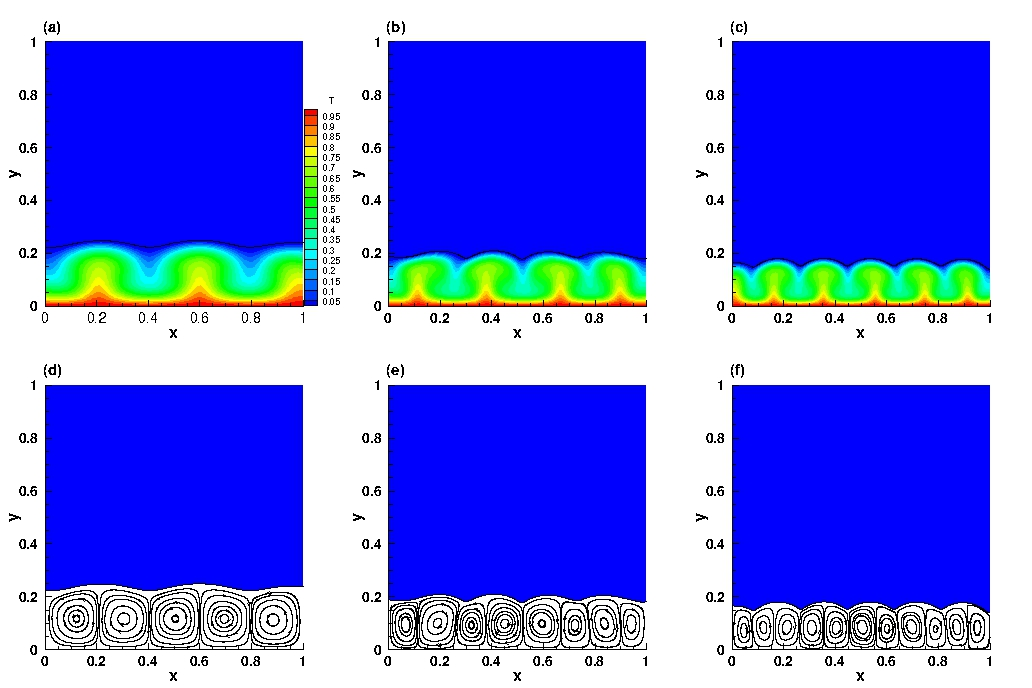
\includegraphics[width=\textwidth]{\figpath/Fig_cap_melting_basal/T_MELT_BASAL_heating_2}
	\end{center}
	\caption{Melting of PCM heated from below: Temperature field and solid-liquid interface for different size of the domain. (a) $\Ray = 3.27 \cdot 10^5$ and $t=30$, (b)  $\Ray = 1.62 \cdot 10^6$ and $t=15$, (c) $\Ray = 3.27 \cdot 10^6$ and $t=10$.}
	\label{fig:melt-below}
\end{figure}

It is useful to introduce the effective Rayleigh and Nusselt numbers of the fluid layer, based on the height of the melting PCM, to describe the temporal evolution of the melting:

\begin{eqnarray}
	Ra_{e} &=& Ra \times \bar {\delta_H}^3, \\
	N\!u_{e} &=& N\!u \times \bar{\delta_H},
\end{eqnarray}
with $\bar{\delta_H}$ the averaged fluid height. Note that $\bar{\delta_H}$ here can be assimilated to the liquid fraction.
In the limit of vanishing $\Ste$ number, the classical no-slip Rayleigh-B�nard convection predicts a critical Rayleigh number $\Ray_c \approx 1707.76 $ \citep{chandrasekhar2013hydrodynamic} after which the first instability appears and the melting front becomes non-planar.
This critical value is increased for increasing values of $\Ste$.
In our simulations, the convective onset occurs at around $\Ray_e \approx 3 \times 10^3$, which is in good agreement with the observation of \cite{esfahani2018basal,favier2019rayleigh}.

\begin{figure}
	\begin{center}
		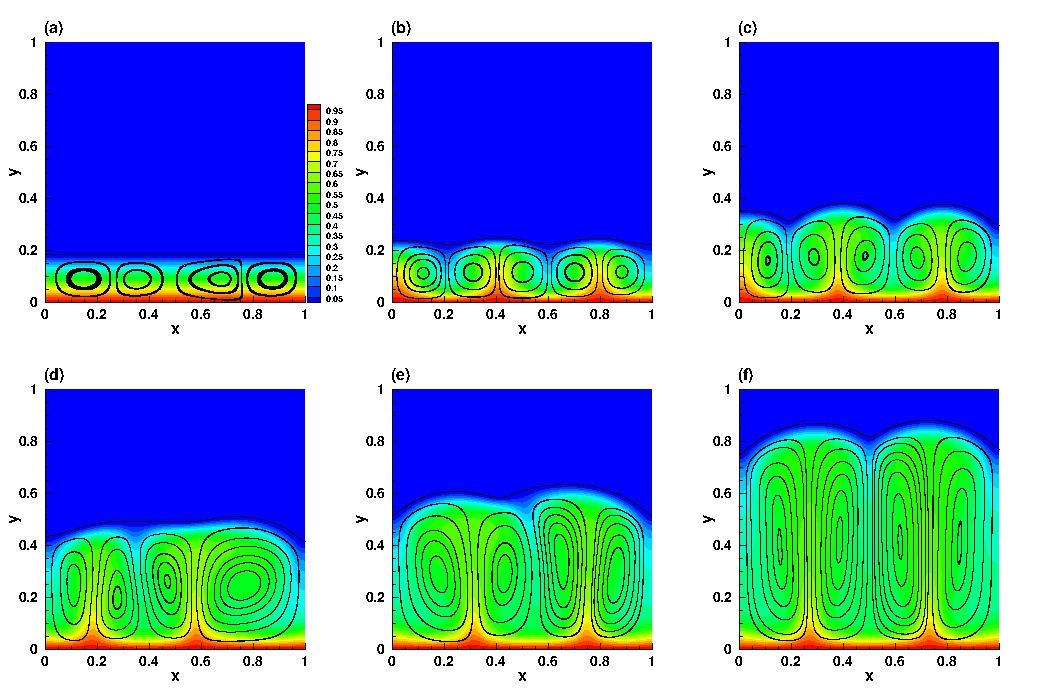
\includegraphics[width=\textwidth]{\figpath/Fig_cap_melting_basal/T_evol_Ra-327e5}
	\end{center}
	\caption{Melting of PCM heated from below: Temperature field and solid-liquid interface for different size of the domain. (a) $\Ray = 3.27 \cdot 10^5$ and $t=30$, (b)  $\Ray = 1.62 \cdot 10^6$ and $t=15$, (c) $\Ray = 3.27 \cdot 10^6$ and $t=10$.}
	\label{fig:T-evol-Ra-3.27e5}
\end{figure}

The time evolution of the melting for $\Ray = 3.27 \times 10^5$ is illustrated in details in Fig. \ref{fig:T-evol-Ra-3.27e5} in panels (a) to (f).
Before the first instability arise, the melt layer evolves solely by conduction. 
There is no noticeable fluid flow and the melting front remains straight (panel (a)).
The convective onset occurs at around $\Ray_e \approx 3 \times 10^3$ and the phase-change interface becomes non-planar (panel (b)).
The appearance of convection is marked by a change in the shape of the interface from straight to nearly periodic curve.
While the fluid depth increases, the effective Rayleigh number increases and the convective rolls are stretched vertically (panels (b) and (c)).
We note that during this stage, the number of rolls is time-independent.
This stage can be compared to the steady convection after the onset in the Rayleigh-B�nard system.
After the rolls are elongated vertically, they start to oscillate laterally and then merge to create greater rolls (panels (d) and (e)).
The essential consequence of the foregoing observation is that the melting front is modified.
The interface is actually shaped by the new flow pattern. 
Two peaks are observed but is still periodic at the interface related to the four convective rolls.
The foregoing steady convection observation is then observed again after the rolls have merged (panel (f)).

\begin{figure}
	\begin{center}
		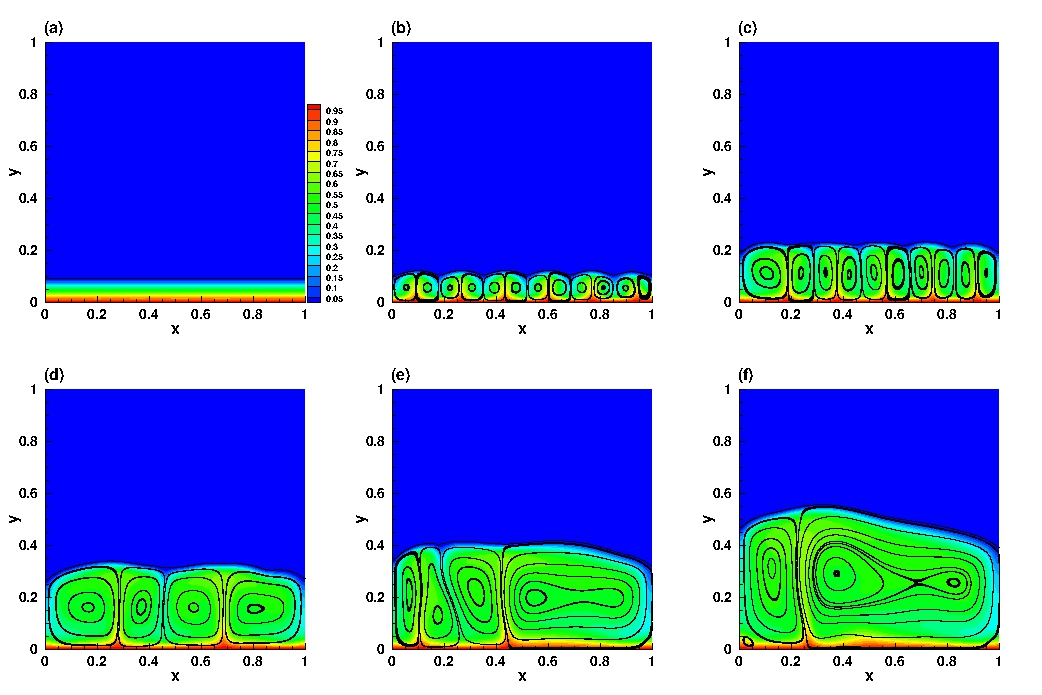
\includegraphics[width=\textwidth]{\figpath/Fig_cap_melting_basal/T_evol_327e6_1}
		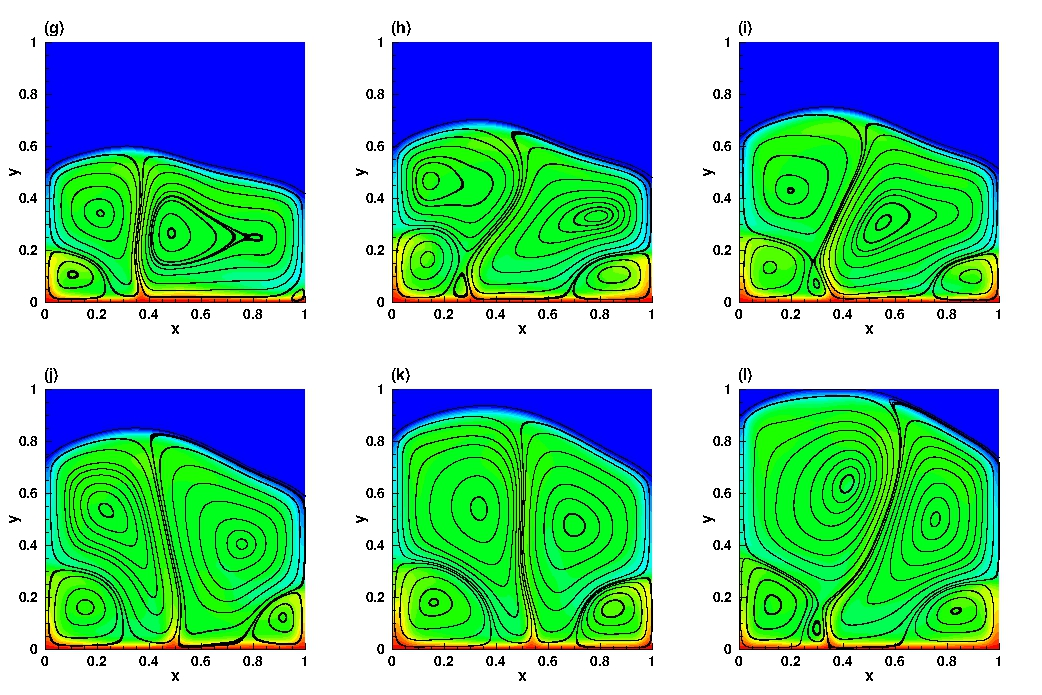
\includegraphics[width=\textwidth]{\figpath/Fig_cap_melting_basal/T_evol_327e6_2}
	\end{center}
	\caption{Melting of PCM heated from below: Temperature field and solid-liquid interface for different size of the domain.$\Ray = 3.27 \cdot 10^6$}
	\label{fig:T-evol-Ra-3.27e6}
\end{figure}

Fig. \ref{fig:T-evol-Ra-3.27e6} shows the dynamic of the melting for higher $\Ray$ number.
The size of the cavity is increased of an order of three, corresponding to $\Ray = 3.27 \times 10^6$ while the $\Ste$ number remains the same.
The stages described previously are recovered in panels (a) to (d).
At $\Ray_e = 4 \times 10^5$ the interface loses periodicity and becomes smoother without cusps (panels (e) and (f)).


\begin{figure}
	\begin{center}
		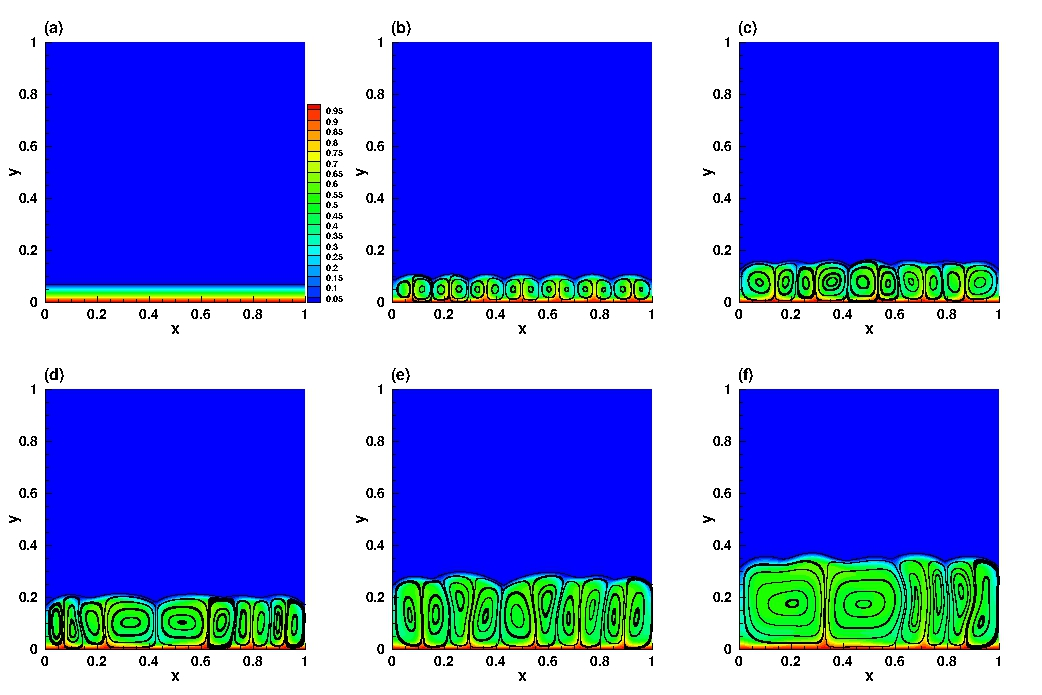
\includegraphics[width=\textwidth]{\figpath/Fig_cap_melting_basal/T_evol_654e6_1}
		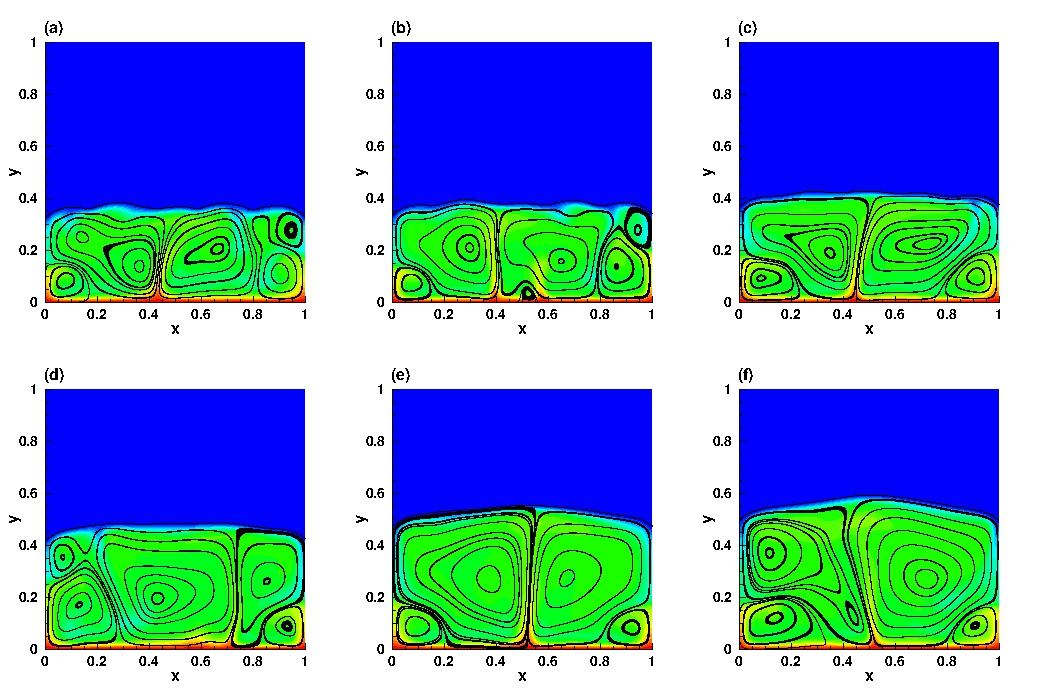
\includegraphics[width=\textwidth]{\figpath/Fig_cap_melting_basal/T_evol_654e6_2}
	\end{center}
	\caption{Melting of PCM heated from below: Temperature field and solid-liquid interface for different size of the domain. (a) $\Ray = 3.27 \cdot 10^5$ and $t=30$, (b)  $\Ray = 1.62 \cdot 10^6$ and $t=15$, (c) $\Ray = 3.27 \cdot 10^6$ and $t=10$.}
	\label{fig:T-evol-Ra-6.54e6}
\end{figure}

\subsection{Scale analysis} \label{sec-RB-scal-analysis}

The previous observation can be assessed more quantitatively by evaluating the heat transfert rate during the melting.
Fig. \ref{fig:NU-LF-evol}(a) plots the temporal evolution of the heat flux represented by the Nusselt number and the strength of buoyancy represented by the Rayleigh number when the melting evolve.
The onset of the convection arises at $\Ray_e = 3 \times 10^3$ when a sudden jump in $N\!u_e$ is observed.
\cite{vasil2011dynamic} have investigated a weakly non-linear stability analysis and have highlighted a superexponentional amplitude growth when the Rayleigh number becomes close to the traditional critical value in the limit of vanishing Stefan number.
This superexponential growth is moreover followed by a rapid pattern readjustment.
The trend of $N\!u_e$ at the onset of convection is in total accordance with the foregoing prediction of \cite{vasil2011dynamic}.
The results of \citep{esfahani2018basal,madruga2018dynamic,favier2019rayleigh} exhibit the same behaviour despite the different conditions (periodic lateral boundary conditions, adiabatic boundary conditions at the top of the cavity and low value of $\Pr$ for \cite{esfahani2018basal} and \cite{favier2019rayleigh}.
The rapid growth of $N\!u_e$ is followed by a power law with averaged smaller exponent $N\!u \sim \Ray^{0.28}$.
Within the framework of natural convection, the Grossmann-Lohse theory \citep{grossmann2000scaling} predicts a scaling exponent of $2/7$ for $10^5 \leq \Ray \leq 10^{14}$.
Our results match remarkably well with this power-law evolution of $N\!u \sim \Ray^{2/7}$.
The transition from steady pattern of the convective rolls to oscillating patterns followed by cell merging, as it is clearly shown in Figs. \ref{fig:T-evol-Ra-3.27e6}(d-f) and \ref{fig:T-evol-Ra-6.54e6}(c-f), 
is also illustrated by a decrease of $N\!u$ at $\Ray \sim 10^5$ followed by high oscillation in the temporal evolution of the heat transfert.
The power-law relation Nu-Ra is bounded in this stage by the average exponent of $1/3$.

One can introduce the following scaling for the time evolution of the liquid fraction.
\begin{equation}\label{eq:scal-Lf-RB}
	L_f(t) = \left[ \sqrt{2 \tau}^{(2-3 \beta)}+ c \Ray^\beta \tau \right]^{1/(2-3 \beta)},
\end{equation}
 with $\beta$ the exponent in the Nu-Ra power law, $c = \frac{(2-3 \beta) \gamma}{2 + \Ste}$ and $\gamma$ a constant fitted from numerical data.
The time evolution of the liquid fraction is illustrated in Fig. \ref{fig:NU-LF-evol}(b).
As expected, the purely diffusive stage displays the scaling $L_f \sim t^{1/2}$.
By replacing $\beta$ by the exponent value $2/7$ in eq. (\ref{eq:scal-Lf-RB}), we obtain $L_f \sim t^{7/8}$.
Our simulations exhibit a power-law evolution of $L_f \sim t^{0.82}$ when the convection is fully developed in the fluid, corresponding to $\Ray_e \geq \Ray_c$.


\begin{figure}
	\begin{center}
		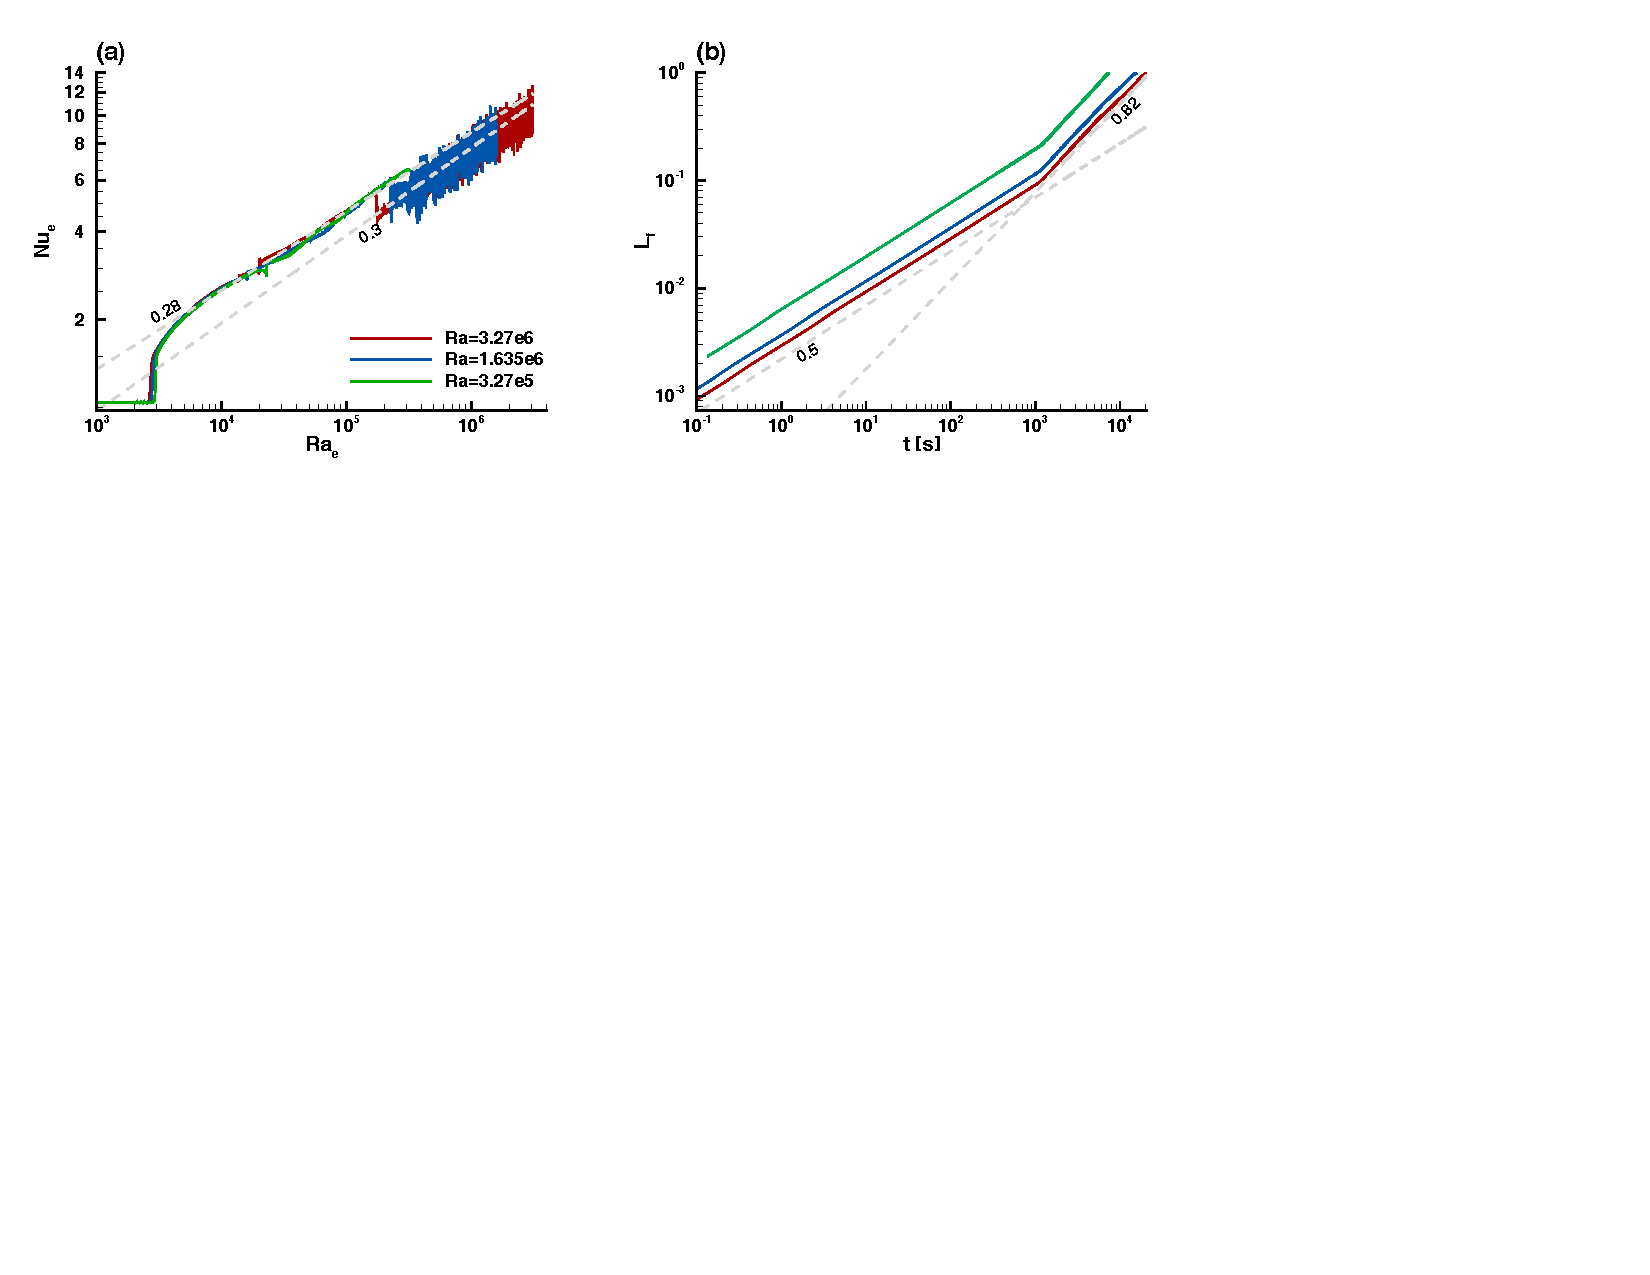
\includegraphics[width=\textwidth]{\figpath/Fig_cap_melting_basal/NU-LF-PHYS}
	\end{center}
	\caption{Melting of PCM heated from below: Temperature field and solid-liquid interface for different size of the domain. (a) $\Ray = 3.27 \cdot 10^5$ and $t=30$, (b)  $\Ray = 1.62 \cdot 10^6$ and $t=15$, (c) $\Ray = 3.27 \cdot 10^6$ and $t=10$.}
	\label{fig:NU-LF-evol}
\end{figure}
